 
\documentclass[12pt]{book}
\usepackage[paper=letterpaper,margin=2cm]{geometry}
\usepackage{amsmath}
\usepackage{amsthm} %needed for the proofs 
\usepackage{amssymb}
\usepackage{amsfonts}
\usepackage{newtxtext, newtxmath}
\usepackage{enumitem}
\usepackage{titling}
\usepackage{titlesec}
\usepackage[english]{babel}
\usepackage{thmtools}
\usepackage{blindtext}
\usepackage{hyperref}
\usepackage{geometry}
\geometry{margin=1.5in}
\usepackage{blindtext}

%For plots
\usepackage{pgfplots}
\pgfplotsset{compat = newest}

\titleformat{\section}
{\normalfont\Large\bfseries}{\thesection}{1em}{}

\newtheorem{theorem}{Theorem}[section]
\theoremstyle{definition}
\newtheorem{definition}{Definition}[section]
\theoremstyle{remark}
\newtheorem*{remark}{Remark}
\newtheorem{corollary}{Corollary}[theorem]
\newtheorem{lemma}[theorem]{Lemma}
\declaretheoremstyle{example}
\declaretheorem[numberwithin=section, style=example, name=Example]{example}
\declaretheoremstyle{proposition}
\declaretheorem[numberwithin=section, style=proposition, name=Proposition]{proposition}
\declaretheorem[numberwithin=section, name=Note]{note}
\declaretheoremstyle{note}

\newcommand\sol{%
  \\ 
  \\
  \textit{Solution:}\\%
}

\hypersetup{
    colorlinks=true,
    linkcolor=blue,
    filecolor=magenta,      
    urlcolor=cyan,
    pdftitle={Overleaf Example},
    pdfpagemode=FullScreen,
    }

\urlstyle{same}

\begin{document}
\begin{titlepage}
	\centering
	{\scshape McGill University \par}
	\vspace{1cm}
	{\scshape\Large Honours Vector Calculus - MATH 248\par}
	\vspace{1.5cm}
	{\huge\bfseries Lecture Notes\par}
	\vspace{2cm}
	{\Large\itshape Alexandre St-Aubin\par}
	\vfill
	Taught by \par
	Niky \textsc{Kamran}

	\vfill

% Bottom of the page
	{\large \today\par}
\end{titlepage}

\tableofcontents
\chapter{Introduction}

\begin{definition}(Scalar Product)
  $$
    \| \overrightarrow{x} \| := \sqrt{ \overrightarrow{x} \cdot \overrightarrow{x}} = \sqrt{\sum^n_{i =1} x_i^2} 
  $$
  $$ \overrightarrow{x} \cdot \overrightarrow{y} = \sum^n_{i=1} x_i y_i = \|\overrightarrow {x}\| \| \overrightarrow{y}\| \cos \theta$$ 
\end{definition} 

\begin{note} $\theta = \cos^{-1} \left(  \frac{\vec{{x}} \cdot \vec{{y}}}{\|\vec{{x}} \| \|\vec{{y}} \| } \right)$
  
\end{note}
\begin{note}
  $ \vec{{x}} \cdot \vec{{y}} = \vec{{y}} \cdot {\vec{{x}} {}}$
\end{note}
\begin{note} 
  If the angle $\theta$  between two vectors is obtuse, then $sign(\theta) < 0$, else $sign(\theta)>0$. 
\end{note}
\begin{theorem} [Cauchy-Shwarz inequality] \label{Cauchy-Shwarz}
  $\forall \vec{{x}}, \vec{{y}} \in \mathbb{R}^n$, 
  $$|\vec{{x}} \cdot \vec{{y}}| \leq \|\vec{{x}} \| \| \vec{{y}} \|
$$
\end{theorem}
\begin{corollary} [Triangle inequality]
  $\forall \vec{{x}} , \vec{{y}} \in \mathbb{R}^n $,
  $$\|\vec{{x}} + \vec{{y}} \| \leq \| \vec{{x}} \| + \| \vec{{y}} \| $$
\end{corollary}
\begin{definition}[Cross product]
  $$\mathbb{R}^3 \times \mathbb{R}^3 \rightarrow \mathbb{R}^3$$
    $$(\vec{{x}} \times \vec{{y}} ) \mapsto \vec{{x}} \times \vec{{y}} = \vec{{n}} $$
    where $\vec{{x}} \times \vec{{y}} = \| \vec{{x}} \| \| \vec{{y}} \| \cdot \sin \theta $ represents the oriented area of the parallelogram spanned by $\vec{{x}}$ and $\vec{{y}}$.  
\end{definition}
\begin{corollary}
  $$ \vec{{x}} \times \vec{{y}} = 0 \iff \vec{{x}}, \vec{{y}} \text{ are linearly dependant. } $$
\end{corollary}
\begin{note} 
  $$\vec{{x}} \times \vec{{y}} = \begin{vmatrix}
    \hat{i} & \hat{j} & \hat{k} \\ 
    x_1 & x_2 & x_3 \\ 
    y_1 & y_2 & y_3 
  \end{vmatrix}  = \hat{i} (x_2y_3 - x_3 y_2) - \hat{j} (x_3 y_1-x_1 y_3 ) + \hat{k} (x_1 y_2 - x_2y_1) $$   
\end{note}

\chapter{Differentiation}
\section{Geometry of real valued functions}%
  \label{sub:Name}
  $f : U \subseteq \mathbb{R}^k \rightarrow \mathbb{R}$

  \begin{example}[i]
    $n =2$, $f(x,y) = x^2 + y^2$, $U = \mathbb{R}^2$
    \newline 
    Paraboloid of revolution:
    \newline
    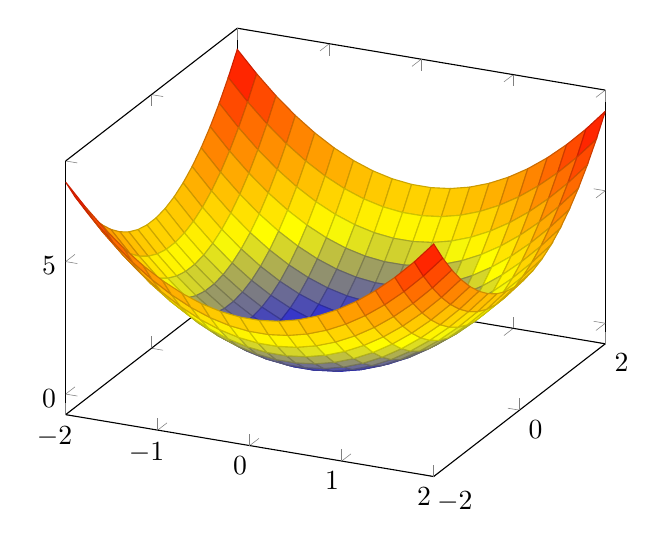
\begin{tikzpicture}
      \begin{axis}[samples=20]
        \addplot3[surf, domain=-2:2] {x^2+y^2};
      \end{axis}
    \end{tikzpicture}

  \end{example}
  
  \begin{example}[ii]
    $n = 2$, $f(x,y) = x^2 + y^2$, $U = \mathbb{R}^2$
    \newline
    Parabolic cylinder:
    \newline
    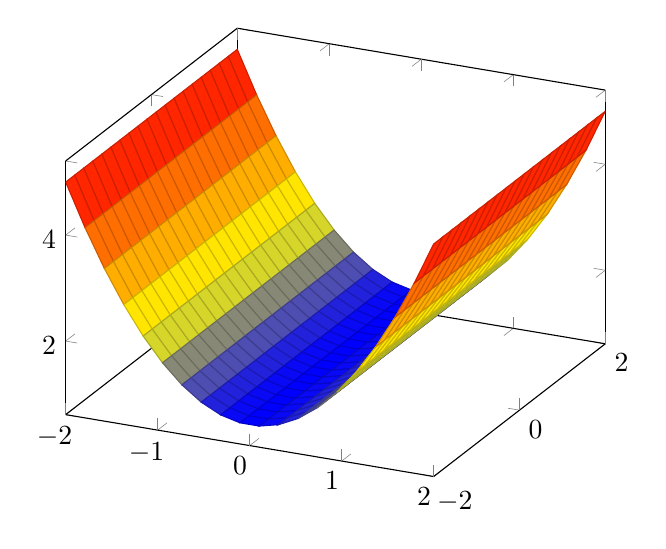
\begin{tikzpicture}
        \begin{axis}[samples=20]
          \addplot3[surf, domain=-2:2] {x^2+1};
        \end{axis}
    \end{tikzpicture}
    
  \end{example}
  \begin{example}[iii]
    $f(x,y) = - \sqrt{1 - x^2 -y^2}$, $ U = \{ (x,y) \mid x^2+y^2 \leq 1 \} $
    \newline
    Southern hemisphere: 
    \newline 
    
    %\begin{tikzpicture}
    %    \begin{axis}[samples=20]
     %     \addplot3[surf, domain=-2:2] {-sqrt(1 - x^2 -y^2)};
    %    \end{axis}
    %  \end{tikzpicture}
  \end{example}

  \begin{definition}[Level set of a function - Inverse image]
    \href{https://mathinsight.org/level_sets#:~:text=For%20a%20function%20of%20three,x%2Cy%2Cz).}{Explanation of level sets}\newline 
    $f: U \subseteq \mathbb{R}^n \rightarrow \mathbb{R}$, $(x_1, ... , x_n) \mapsto f(x_1, ... , x_n)$. Let $c \in \mathbb{R}$, then the \textit{level set} corresponding to $c$ is the set of points in the domain where $f(x_1, ..., x_n) = c$, that is,
    $$ L_c (f) = \{ (x_1, ..., x_n) \mid f(x_1, ..., x_n) = c \} $$
    And,
    $$ f^{-1}(\{c\})\subset U \subseteq \mathbb{R}^n $$  
  \end{definition}
  \begin{example}[ii]
    $n =3, \; (x,y,z)f(x,y,z) = x^2 + y^2 +z^2$
    \newline
    $$L_{-1}= \{ (x,y,z) \mid x^2 +y^2 + z^2 = -1 \}= \emptyset$$
    $$L_0 =  \{ (x,y,z) \mid x^2 + y^2 + z^2 = 0 \} = (0,0,0)$$
    $$L_{15} =  \{ (x,y,z) \mid x^2 + y^2 + z^2 = 15 \} = \text{sphere of radius }\sqrt{15} $$ 
 \end{example} 

\begin{example}[iii]
  $f(x,y,z) = x^2 -y^2 +z^2$
  $$L_1 =  \{ (x,y,z) \mid x^2 - y^2 + z^2 = 1 \} =\text{hyperboloid of revolution of 1 sheet} $$ 
   $$L_0 =  \{ (x,y,z) \mid x^2 - y^2 + z^2 = 0 \} = \text{cone} $$
   because you get $y = \sqrt{x^2 + z^2}$.
  \newline
  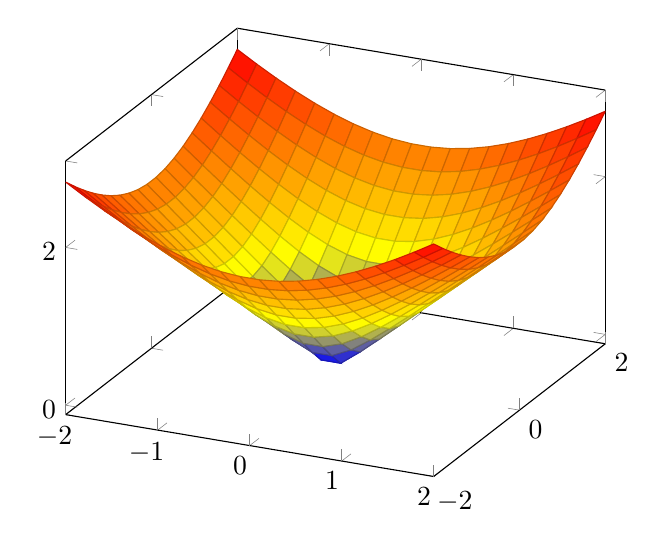
\begin{tikzpicture}
       \begin{axis}[samples=20]
         \addplot3[surf, domain=-2:2] {sqrt(x^2+y^2)};
       \end{axis}
  \end{tikzpicture}
   $$L_{-1} =  \{ (x,y,z) \mid x^2 - y^2 + z^2 = -1 \} =\text{hyperboloid of revolution of 2 sheets} $$ 
\end{example}
\begin{example}[iv]
  level sets of $f:= x^2 -2y^2 +z^2$. 
\end{example}
\section{Limits and continuity}%
  \label{sub:Limits and continuity}
  \begin{definition}
   $D_r (\vec{{x}}) : = \{\vec{{x}}  \in \mathbb{R}^n \mid \| \vec{{x}} - \vec{{x_0}} < r\} = \text{open ball radius $r>0$ centered at $\vec{{x_0}}$ }$.
  
  \end{definition}
  \begin{definition}
    $U\subseteq \mathbb{R}^n$ is \textit{open} if $\forall \vec{{x_0}} \in U, \; \exists r>0 $ s.t. $D_r(\vec{{x_0}}) \subset U$.  
  \end{definition}
  \begin{proposition}
   $D_r(\vec{{x_0}})$ is open. 
  \end{proposition}
  \begin{definition}[Limit]
    Let $f:U\subseteq \mathbb{R}^n \rightarrow \mathbb{R}^m$ be defined over $U$, open in $\mathbb{R}^n$. We say that  $$\lim_{\vec{{x}} \rightarrow \vec{{x}}_0 }f(\vec{{x}}) = \vec{{b}}$$
    if for all $\varepsilon > 0 $, $\exists \delta (\varepsilon, \vec{{x_0}} )$ such that $$\|\vec{{x}} -\vec{{x_0}} \| < \delta \implies \|f(\vec{{x}}) -\vec{{b}}  \| < \varepsilon$$
  \end{definition}
  \begin{definition}
    $f$ is \textit{continuous} at $\vec{{x_0}} \in U$ if $\lim_{\vec{{x}} \rightarrow \vec{{x_0}} } f(\vec{{x}} ) = f(\vec{{x_0}})$ 
\end{definition}
\begin{proposition}

\begin{enumerate}$  $
  \item $\lim (f \pm g) = \lim f \pm \lim g$ 
  \item $\lim (f\cdot g) = \lim f \cdot \lim g$
  \item $\lim (f / g) = \frac{\lim f}{\lim g}$ if $\lim g \neq 0$ 
\end{enumerate}
\end{proposition}
\begin{example}
  Let $f(x,y) = x+y$. Show that $\lim_{(x,y) \rightarrow (x_0, y_0)} f(x,y) = x_0 +y_0$ using the $\varepsilon -\delta$ definition.
\end{example}
\begin{example}
  Show that $\lim_{(x,y)\rightarrow (0,0)}\frac{4x^2y}{x^2+y^2} = 0$. 
  \begin{proof}
    We want to show that $$\|\vec{{x}} -(0,0)\| = \| \vec{{x}} \| <\varepsilon \implies \left| \frac{4x^2y}{x^2 + y^2}-0\right|<\delta $$
  Let $\varepsilon = \frac{\delta}{4}$, then

\begin{equation*}
	\begin{split}
	   \|\vec{{x}} \| < \varepsilon \implies &  \sqrt{x^2 + y^2}<\frac{\delta}{4} \\ 
    \implies & \sqrt{y^2} < \frac{\delta}{4} \\ 
   	\implies & 4y < \delta\\
    \implies & \delta > 4|y| = \left|\frac{4x^2y}{x^2} \right| > \left|\frac{4x^2y}{x^2+ y^2} \right| \\
	\end{split}
\end{equation*}
  \end{proof}
  \end{example}
  \begin{example} 
    Show that $\lim_{(x,y) \rightarrow (0,0)} \frac{x^2y^2}{x^2+y^2} = 0$. 
    \begin{proof} 
      Need to estimate $\frac{x^2y^2}{x^2 + y^2} $ in terms of $\| \vec{{x}} -(0,0)\| = \sqrt{x^2 + y^2}$. 
      \begin{equation*}
        \begin{split}
          \left| \frac{x^2y^2}{x^2 + y^2}\right| = |x^2 | \cdot \left| \frac{y^2}{x^2 +y^2}\right| \leq x^2 < x^2 +y^2
        \end{split}
      \end{equation*}
      And, if $\| \vec{{x}} -(0,0) \| = \sqrt{x^2 +y^2} < \delta$, then $\left| \frac{x^2y^2}{x^2 +y^2}\right|< \delta^2$. Hence, take $\delta = \sqrt{\varepsilon}$
    \end{proof}
    
  \end{example}
  \begin{example}
    $f(x,y) = \left\{ \begin{matrix} \frac{xy^3}{x^2 +y^6} & \text{if } (x,y) \neq (0,0) \\ 
      0 & \text{if } (x,y) = (0,0)
    \end{matrix}
      \right. $
      show that $f$ is not continuous at (0,0). 
      \begin{proof} 
        $$ \lim_{y \rightarrow 0} f(0,y) = \frac{0}{0+y^6} = 0 \quad \text{ with  }y \neq 0 $$
        Now, 
        $$f(y^3, y) = \frac{y^3-y^3}{y^6+y^6} =\frac{y^6}{2y^6}  $$
        and $$\lim_{y \rightarrow 0} f(y^3,y) =\frac{1}{2}  $$
        So, since the limits are different, $f$ is not continuous. 
      \end{proof} 
  \end{example}
  \begin{example}
    $\lim_{(x,y) \rightarrow (0,0)} \frac{\sin(xy)}{xy} = 1$
    \begin{proof} 
      Let $f=\frac{\sin(xy)}{xy}$, $(x,y) \mapsto t = xy$ is continuous , $t \mapsto \frac{\sin t }{t} $. $$\lim_{(x,y) \rightarrow (0,0)}xy = 0 $$
      and by recall, $$\lim_{(x,y) \rightarrow (0,0)} \frac{\sin (xy)}{xy} = 1 $$
    \end{proof}
    
  \end{example}
  \section{Differentiation}
  $f: (x_1, ..., x_n) \mapsto f(x_1,...,x_n)$, $\vec{{x_0}} \in U =$ domain of $f$. $$\left. \frac{\partial f}{\partial x_i}\right|_{\vec{{x_0}} } := \lim_{h \rightarrow 0} \frac{f(\vec{{x_0}} + h \vec{{e_i}} -f(\vec{{x_0}} ))}{h}   $$

  Want $f: U \subseteq \mathbb{R}^n \rightarrow \mathbb{R}^m$, $\vec{{x_0}} \in U $, $(Df)(\vec{{x_0}})$ (derivative of $f$ at $\vec{{x_0}}$, linear map )
  \newline
  \begin{definition}Linear approximation of $f$ at $\vec{{x_0}}  =x_0$, $ \left. lf \right|_{\vec{{x_0}}} : \mathbb{R}\mapsto \mathbb{R}$ is  
    \begin{equation*}
      \begin{split}
        \left. Lf \right|_{x_0} := f(x_0) + f^\prime (x_0)(x-x_0)
      \end{split}
    \end{equation*}
    That is, the linear approximation is the graph of the tangent line at $x_0$.
    
  \end{definition}
  \begin{definition}$ \left. Lf \right|_{\vec{{x_0}}}: \mathbb{R}^2 \mapsto \mathbb{R} $
    \begin{equation*}
      \begin{split}
        \left. Lf \right|_{(x_0, y_0)} (x,y) = f(x_0,y_0) + \frac{\partial f}{\partial x} (x_0, y_0) (x-x_0) + \frac{\partial f}{\partial y} (x_0, y_0) (y-y_0) 
      \end{split}
    \end{equation*}
    
  \end{definition}
  \begin{example}$f(x,y) = -\sqrt{1-x^2-y^2}$, let $(x_0, y_0) = (\frac{1}{\sqrt{3}}, \frac{1}{\sqrt{3}})$. 
   \newline 
    $$f(x_0, y_0) = -\frac{1}{\sqrt{3}}  $$
    $$\frac{\partial f}{\partial x} =- \frac{-2x}{2\sqrt{1-x^2 -y^2}} = \frac{x}{\sqrt{1-x^2-y^2}}   $$
    And, 
    \begin{equation*}
      \begin{split}
        \frac{\partial f}{\partial x} \left( \frac{1}{\sqrt{3}} , \frac{1}{\sqrt{3}}  \right) = \frac{\frac{1}{\sqrt{3}} }{\sqrt{1 - 2/3}} = 1 
      \end{split}
    \end{equation*}
    So, 
    \begin{equation*}
      \begin{split}
        \left. Lf \right|_{( \frac{1}{\sqrt{3}} , \frac{1}{\sqrt{3}} )} (x,y) = -\frac{1}{\sqrt{3}}+ 1(x - \frac{1}{\sqrt{3}} ) +1(x - \frac{1}{\sqrt{3}} )= x+y- \sqrt{3} 
      \end{split}
    \end{equation*}
  \end{example}
    We need more than the existence of partial derivatives $\frac{\partial f}{\partial x_i}(\vec{{x_0}} {}) $ to conclude for example that $f$ is continuous at $\vec{{x_0}}.$ We need \textit{Differentiability}! 
    \begin{definition}(Differentiability). $f: U\subseteq \mathbb{R}^n \rightarrow \mathbb{R}^m$ is differentiable at $\vec{{x_0}} $ if \begin{equation*}
      \begin{split}
        \lim_{\vec{{x}} \rightarrow \vec{{x_0}} }\frac{\|f(\vec{{x}}) -Lf|_{\vec{{x_0}}} (\vec{{x_0}}) \|}{\| \vec{{x}} -\vec{{x_0}} \|} = 0
      \end{split}
    \end{equation*}
    \end{definition}
    \begin{theorem} 
      $f$ is differentiable at $\vec{{x_0}} \implies$ $f$ is continuous at $\vec{{x_0}} $. 
    \end{theorem}
    However, the existence of $\frac{\partial f}{\partial x}(x_0,y_0) $ and $\frac{\partial f}{\partial y} (x_0, y_0)$ DOES NOT imply that $f$ is continuous at $(x_0, y_0)$. 
    \begin{example}
      $f(x,y) = \left\{\begin{matrix}\frac{xy}{x^2+y^2} , & (x,y) \neq (0,0) \\ 0, & \text{o.w.} \end{matrix} \right. $
     \newline 
      CLAIM: 
      \begin{equation*}
        \begin{split}
          \frac{\partial f }{\partial x} (0,0) = \lim_{h \rightarrow 0}\frac{f(h,0) - f(0,0)}{h}= 0 \\ 
          \frac{\partial f }{\partial y} (0,0) = 0
        \end{split}
      \end{equation*}
      but $f$ is discontinuous at $(0,0)$. 
      \begin{proof} 
        \begin{equation*}
          \begin{split}
            f(x,y) = \frac{x^2}{x^2+ x^2} \implies \lim_{x \rightarrow 0} f(x,x) = 1/2 
          \end{split}
        \end{equation*}
        but, 
        \begin{equation*}
          \begin{split}
            \lim_{x \rightarrow 0} f(x, 0) = 0
          \end{split}
        \end{equation*}
        Hence, since the limits differ, the function is discontinuous.
      \end{proof}
    \end{example}
    \begin{theorem} \label{}
      $ \frac{\partial f }{\partial x},  \frac{\partial f }{\partial y} $ continuous at $(x_0, y_0) \implies f$ is differentiable at $(x_0, y_0)$.
    \end{theorem}
    \begin{definition}[Component functions] 
      Consider a function $r(t) = \begin{bmatrix} f(t)\\ g(t) \end{bmatrix}$, which has one variable for input and a vector for output is called single-variable vector-valued functions. The functions $f (t)$ and $g(t)$ are the \textbf{component functions} of $r(t)$. They are each a single-variable real-valued function.      
    \end{definition}
    \begin{example}
      $r(t) = \begin{bmatrix} \sin t \\ \cos t\end{bmatrix}$, $\sin t$ and $\cos t$ are the component functions of $r(t)$. 
    \end{example}
    \begin{definition}
      $(Df) (\vec{{x_0}})$ is the derivative linear map represented by 
      \begin{equation*}
        \begin{split}
          Df = \begin{pmatrix} \frac{\partial f_1}{\partial x_1} &\hdots &  \frac{\partial f_1}{\partial x_n} \\ 
            \vdots & \ddots &\vdots \\ 
            \frac{\partial f_m}{\partial x_1} & \hdots &  \frac{\partial f_m}{\partial x_n}  
          \end{pmatrix}
        \end{split}
      \end{equation*}
      Where $f_i$ are the component functions of $f$. 
      
    \end{definition}
    \begin{example}It is possible for $f(x,y)$ to be continuous at $(x_0, y_0)$, for $\frac{\partial f}{\partial x} , \frac{\partial f}{ \partial y } $ to exist at $(x_0, y_0)$, but for $f$ not to be differentiable at $(x_0, y_0)$. 
      \begin{proof} 
        consider $f: \mathbb{R}^2 \rightarrow \mathbb{R},$ $(x,y) \mapsto (xy)^{1/3} $. $f$ is continuous at $(0,0)$. And, 
        \begin{equation*}
          \begin{split}
            \frac{\partial f}{\partial x} (0,0) = \lim_{h \rightarrow 0}\frac{f(h,0)- f(0,0)}{h} =0
          \end{split}
        \end{equation*}
        The partial wrt $y$ is equal to 0 likewise.  But, 
        \begin{equation*}
          \begin{split}
            \lim_{(x,y) \rightarrow (0,0)} \frac{|f(x,y) - (f(0,0)+ Df(0,0)(x,y))|}{\| (x,y)-(0,0) \|} =   \lim_{(x,y) \rightarrow (0,0)} \frac{|(xy)^{1/3} - 0 |}{\sqrt{x^2 + y^2}} 
          \end{split}
        \end{equation*}
      \end{proof}
    \end{example}
    \begin{lemma} $(Df)(\vec{{x}} )$ continuous at $\vec{{x_0}}\implies f$ is differentiable at $\vec{{x_0}} $ 
    \end{lemma}
    \section{ Paths and Curves }
    \begin{example}
      $\vec{{c}} (t) = (t,t)$, $0<t<1$      
    \end{example}
    \begin{example}
      $\vec{{c}} (t) = (t^2, t^2)$
    \end{example}
    The two examples above are different parametrized curves, but the paths covered are the same. 
    \begin{example}
      $\vec{{c}} (t) = (a \cos t , b \sin t , t)$, $- \infty < t < \infty$, $ a > 0, b> 0 $. This is an elliptic helix (circular if $a = b$). 
    \end{example}
    \begin{lemma} 
      Tangent line to the path of $\vec{{c}} (t)$ at $\vec{{c}} t_0$ is $$\vec{{l}} (t) = \vec{{c}} (t_0)+ \vec{{c}}^\prime (t_0)(t-t_0) $$ 

    \end{lemma}
    \section{Properties of the derivative}
    \begin{theorem}$ $ 
      \begin{enumerate}
        \item $D(f\pm g) = Df \pm Dg$
        \item $m = 1,$ $D(fg) = (Dfg + fDg)$ (leibniz rule)
        \item $D\left(\frac{f}{g}\right) = \frac{Dfg - fDg}{g^2} $, provided $g(\vec{{x_0}}) \neq 0)$
      \end{enumerate}
    \end{theorem}
      \begin{theorem}(Chain rule)
        $\mathbb{R}^n \overset{f}{\rightarrow} \mathbb{R}^m \overset{g}{\rightarrow} \mathbb{R}^p$, $f$ is differentiable at $\vec{{x_0}}$, $g$ differentiable at $f(\vec{{x_0}})$. 
        \begin{equation*}
          \begin{split}
            D(g \circ f)(\vec{{x_0}}) = (Dg)(f(\vec{{x_0}} ))\cdot (Df)(\vec{{x_0}} )
          \end{split}
        \end{equation*}
        where $\cdot$ is the composition of linear maps; matrix product.  
      \end{theorem}
      \begin{theorem} \label{Chain Rule (General Version)}
        Suppose that $u$ is a differentiable function of the $n$ variables $x_1,..., x_n$ and each $x_j$ is a differentiable function of the $m$ variables $t_1, ..., t_m.$ Then $u$ is a function of $t_1,..., t_m$ and 
        $$ \frac{\partial {u}}{\partial {t_i}} = \frac{\partial {u}}{\partial {x_1}} \frac{\partial {x_1}}{\partial {t_i}} + \hdots + \frac{\partial {u}}{\partial {x_n}} \frac{\partial {x_n}}{\partial {t_i}} {} $$
      \end{theorem}
      \begin{example}
        $n = p = 1$, $\mathbb{R}\rightarrow \mathbb{R}^m \rightarrow \mathbb{R}$, $t \mapsto (x_1, ..., x_m )\mapsto u$.  
        $$f: t \mapsto (x_1(t), ... , x_m(t))$$
        $$g: (x_1, ..., x_m) \mapsto u $$
        $$(g \circ f) (t) = g(x_1(t), ...,x_m (t)) $$
        and, 
      \begin{equation*}
        \begin{split}
          \frac{d}{dt} (g \circ f)(t) =&  (Dg)(f(t)) \cdot (Df)(t) \quad [\text{Chain rule}]\\ 
          =& \left(\frac{\partial g}{\partial x_1} ... \frac{\partial g}{\partial x_m}   \right)(\vec{{x}} (t))\cdot \begin{pmatrix} x_1^\prime (t) \\ \vdots \\ x^\prime_m(t)
          \end{pmatrix} \\ 
          =& \frac{\partial g}{\partial x_1}x^\prime_1 + ... + \frac{\partial g}{\partial x_m} x^\prime_m 
        \end{split}
      \end{equation*} 
      \end{example} 
      \begin{example}
        $\mathbb{R}^2 \overset{f}{\rightarrow} \mathbb{R}^2 \overset{g}{\rightarrow} \mathbb{R}$, $(r, \theta) \mapsto (x,y) \mapsto u$, where 
        $$ f: (r, \theta) \mapsto (r\cos \theta, r \sin \theta) $$
        and 
        $$g : (x,y) \mapsto u = g(x,y) $$
        Let $h = g \circ f$, then 
        $$h(r, \theta) = u = g(r\cos \theta, r \sin \theta) $$
        and, 
        \begin{equation*}
          \begin{split}
            Dh = \left( \frac{\partial h}{\partial r} \frac{\partial h}{\partial \theta}  \right) =& (Dg)\cdot (Df)(r, \theta) \\
            =&  \left( \frac{\partial g}{\partial x} \frac{\partial g}{\partial y}  \right) \begin{pmatrix} \frac{\partial f_1}{\partial r} = \cos \theta & \frac{\partial f_1 }{\partial \theta} = -r \sin \theta \\ 
            \frac{\partial f_2 }{\partial \theta} = \sin \theta & \frac{\partial f_2 }{\partial \theta}=r \cos \theta \end{pmatrix} \\ 
            =& \left( \cos \theta \frac{\partial g }{\partial x} + \sin \theta \frac{\partial g }{\partial y} - r \sin \theta  \frac{\partial g }{\partial x} + r \cos \theta \frac{\partial g }{\partial y}\right)
          \end{split}
        \end{equation*}
      \end{example}
      \section{Gradients and directional derivatives}%
        \label{sub:Gradients and directional derivatives}
        $f: U\subseteq \mathbb{R}^n \rightarrow \mathbb{R}$, differentiable. 
        $$(Df)(\vec{{x}} ) = \left(\frac{\partial {f}}{\partial {x_1}} (\vec{{x}} ) ... \frac{\partial {f}}{\partial {x_n}} (\vec{{x_n}} )  \right) := (\vec{{\nabla}}f) (\vec{{x}})\left(\frac{\partial {f}}{\partial {x_1}} (\vec{{x}} ) ... \frac{\partial {f}}{\partial {x_n}} (\vec{{x_n}} )  \right)$$
        \begin{definition}
          $(\vec{{\nabla}}_{\vec{{v}}}f) (\vec{{x}}) : = $
           the directional derivative of $f$ at $\vec{{x}}$ in direction $\vec{{v}}$. 
        \end{definition}
        \begin{definition}[Directional derivative]
          $\frac{d}{dt}|_{t=0} f( \vec{{x}} + t \vec{{v}} )$ is the rate of change of $f$ along the line through $\vec{{x}} $ in direction of $\vec{{v}} $, at the point $\vec{{x}}$.  
        \end{definition}
        \begin{proposition} \label{}
          $(\vec{{\nabla}}_{\vec{{v}}}f) (\vec{{x}}) =  \vec{{v}} (\vec{{\nabla}} f)(\vec{{x}} ) = \sum^{n}_{i=1} v_i \frac{\partial {f}}{\partial {x_i}} (\vec{{x}})$
          \begin{proof} 
            $D$(comp) = comp of $D's$ = $\vec{{v}}\cdot  \vec{{\nabla}}f(\vec{{x}} + t \vec{{v}})$. Set $t = 0$ and we are done.  
          \end{proof}
        \end{proposition}
        \begin{remark} 
            Conventionally, we often assume that $\|\vec{{v}}\| = 1$ and write $\vec{{v}} = \vec{{n}}$.
        \end{remark}
        \begin{example}
          Compute directional derivative of 
          $$f(x,y) = (x^2 + y^2) e^{-(x^2 + y^2 + 10)} $$ 
          at $\vec{{x}} = (2,1)$ in the direction $\vec{{n}}$ corresponding to $\vec{{v}} $ pointing from $(2,1)$ to $(0,0)$. 
          Want to find:
         $ 
              (\vec{{\nabla}}_{\vec{{v}}} f)(2,1) = \vec{{n}} (\vec{{\nabla}}f) ( 2,1 )
            $
          \begin{equation*}
            \begin{split}
              (\vec{{\nabla}}f) =& \left(\frac{\partial {f}}{\partial {x}} , \frac{\partial {f}}{\partial {y}}  \right) \\ 
              \frac{\partial {f}}{\partial {x}} =& e^{-(x^2+y^2 +10)} (2x + (x^2 + y^2 (-2x))) \\ 
              \frac{\partial {f}}{\partial {x}}(2,1) =& -16e^{-15} \\ 
              \frac{\partial {f}}{\partial {y}} =& e^{-(x^2+y^2 +10)} (2y +(x^2+ y^2)(-2y))  \\ 
              \frac{\partial {f}}{\partial {y}}(2,1) =& -8e^{-15} 
            \end{split}
          \end{equation*}
          And, 
          $$\vec{{n}} = \frac{(-2, -1)}{\sqrt{5}}$$
          $$(\vec{{\nabla}}_{\vec{{n}}} f)(2,1) = \frac{e^{-15}}{\sqrt{5}} (32 + 8) = \frac{40 }{\sqrt{5}} e^{-15} $$
        \end{example}
       \subsection{Geometric interpretation of the gradient}%
        \label{sub:Geometric interpretation of the gradient}
         
      \begin{enumerate}
        \item $(\vec{{\nabla}}_{\vec{{n}}}f) (\vec{{x}}) = \vec{{n}} \cdot (\vec{{\nabla}} f) \vec{{x}} =\| \vec{{n}}\| \| \vec{{\nabla }}f(\vec{{x}})\| \cos \theta$. $(\vec{{\nabla}}_{\vec{{n}}}f) (\vec{{x}})$ is the largest when $\theta = 0$, that is when $\vec{{n}}$ is aligned with $(\vec{{\nabla}}f) (\vec{{x}} {})$.
        \item Consider $f: U \subseteq \mathbb{R}^n \rightarrow \mathbb{R}$, $d \in range(f)$. Then the level set of $d:$ $$\mathcal{L}_d = f^{-1}(\{d\}) = \{ (x_1, ..., x_n) \mid f(x_1,...,x_n) = d\} $$
         If $\vec{{x}} \in \mathcal{L}_d$ is such that $(\vec{{\nabla}}f) (\vec{{x}}) \neq 0$  (at least one of the partial derivatives $\frac{\partial {f}}{\partial {x_i}} (\vec{{x}}) \neq 0$) then, $$(\vec{{\nabla}}f)(\vec{{x_0}}) \perp \mathcal{L}_d $$
 It follows that the gradient of the function at any point is normal to the tangent plane at that point to the level surface through that point. This can be exploited to plot the tangent plane to a surface at a chosen point.
 \begin{definition}[Tangent plane to level surfaces]
   Let $S$ be the surface consisting of those $(x,y,z)$ such that $f(x,y,z) = k$, for a constant $k$. The \textbf{Tangent plane} of S at a point $(x_0, y_0, z_0)$ of $S$ is defined by the equation $${{\nabla}}f(x_0 , y_0, z_0 )\cdot (x-x_0, y-y_0, z-z_0) = 0$$ if $\nabla f(x_0, y_0, z_0) \neq 0.$ That is, the tangent plane is the set of points $(x,y,z)$ that satisfy the equation above.  
  
 \end{definition}
        \begin{example}
          $f(x,y) = x^2 + y^2 + 1$
          \newline 
          \begin{center}
          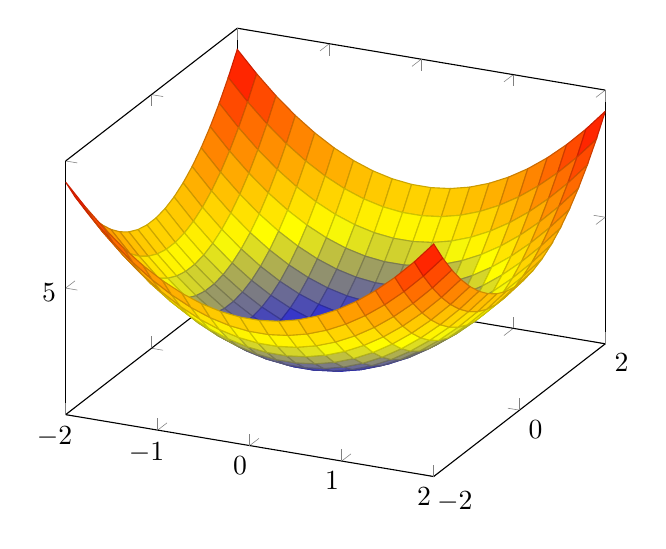
\begin{tikzpicture}
              \begin{axis}[samples=20]
                \addplot3[surf, domain=-2:2] {x^2+y^2+1};
              \end{axis}
            \end{tikzpicture}
          \end{center}
        Let $d \in [1, + \infty)$, 
          $$(\vec{{\nabla}} f) (x,y) = 2(x,y)  $$
          And, $(\vec{{\nabla}} f) (x,y) = \vec{{0}} \iff (x,y) = (0,0)$. Level curves of $f$ : 
          $$x^2 + y^2 +1 = d \implies x^2 + y^2 =d-1 \quad [d>1] $$

          And we obtain $\mathcal{L}_d = $ circles of radius $\sqrt{d-1}$ centered at (0,0). The gradient is always perpendicular to the level set curves, so they are vectors starting at (0,0) and going out of the circle. 
          \begin{center}
            \begin{tikzpicture}
    \draw[->] (-4,0) -- (4,0) node[right] {$x$};
    \draw[->] (0,-4) -- (0,4) node[above] {$y$};
    % Draw the circles centered at the origin
    \draw (0,0) circle (1cm);
    \draw (0,0) circle (2cm);
    \draw (0,0) circle (3cm);

    % Draw the vector \vec{\nabla}f from (0,0) to (1,0)
    \draw[->] (0,0) -- (3,3) node[right] {$\vec{\nabla}f$};
\end{tikzpicture}
          \end{center}
        \end{example}
        

      \end{enumerate}
    Question: Can level sets intersect? No, otherwise $f$ would not be a function.  
    \begin{remark}
      We can use the second geometric interpretation to write the equation of the tangent planes to \textit{Level sets} and \textit{Graphs}. 
    \end{remark} 
    \begin{example}
      Take $n = 3$, $\mathcal{L}_d = \{ (x,y,z) : f(x,y,z) = d  \}$. Let $\vec{{x}}$ the position vector of a point in tangent plane. The equation of the tangent plane is 
      $$(\vec{{x}} -\vec{{x_0}})(\vec{{\nabla}}f)(\vec{{x_0}} )=0$$
      \begin{equation}(x- x_0) \frac{\partial {f}}{\partial {x}} (x_0, y_0, z_0)+ (y-y_0)\frac{\partial {f}}{\partial {y}} (...)+ (z-z_0) \frac{\partial {f}}{\partial {z}} (...) = 0 \end{equation}
    \end{example}

    \begin{example}Now, for the graph of $g(x,y)$. Write it as a level set: 
      $$f(x,y,z) = z - g(x,y) = 0 = d$$
      Rewriting (1) in terms of $g$:
      \begin{equation*}
        \begin{split}
          (x-x_0)\left( -  \frac{\partial {g}}{\partial {x}} (x_0, y_0) \right)+ (y-y_0) \left(- \frac{\partial {g}}{\partial {y}} (x_0, y_0)  \right) + (z - g(x_0 , y_0))\cdot 1 = 0 
        \end{split}
      \end{equation*}
      Or, $$z(x,y) = g(x_0, y_0) + \frac{\partial {g}}{\partial {x}} (x_0,y_0)(x-x_0) + \frac{\partial {g}}{\partial {y}} (x_0, y_0 ) (y-y_0) = Lg|_{(x_0, y_0)} = \text{linear approx.} $$
       
    \end{example}
    \chapter{Higher Order derivatives}%
      \label{sec:Higher Order derivatives}
    \section{Iterated Partial Derivatives}%
      \label{sub:Iterated Partial Derivatives}
      \begin{example}
        let $n = 2$, $\frac{\partial^2 {f}}{\partial {y} \partial x}: = \frac{d}{d y} \left(\frac{d {f}}{d {x}} \right)$ 
        
      \end{example}

      \begin{definition}
        $f$ is of class $C^k(f \in C^k (U))$ if $\frac{\partial^k f}{\partial x_{i_1}...x_{i_k}} $ are continuous in $U$ for all $1\leq i_1,..., i_k \leq n$.  
      \end{definition}
      \begin{remark}
        Notation: $f_x : = \frac{\partial {f}}{\partial {x}} $, and $ f_{xy} : \frac{\partial^2 {f}}{\partial {x} \partial {y}} {} $.
      \end{remark}
\begin{example}[Question] Does the order matter when taking kth order derivatives? yes.
\end{example}
\begin{theorem} (Shwarz) : $f \in C^2 (U) \implies \frac{\partial^2 {f}}{\partial {x_i} \partial {x_j}} = \frac{\partial^2 {f}}{\partial {x_j} \partial {x_i}} {}$ at every point of $U$, likewise for $\frac{\partial^k {f}}{\partial {x_{i_1}}... \partial {x_{i_k}}} {}$.
\end{theorem}
\begin{remark} 
  There exist functions for which $f_{xy} \neq f_{yx}$. For example (Peano): 
  \begin{equation*}
    \begin{split}
      f(x,y) : = \left\{ \begin{matrix}
        \frac{x^3y - xy^3}{x^2 + y^2} & (x,y) \neq (0,0) \\ 
        0 & o.w. 
      \end{matrix} \right.
    \end{split}
  \end{equation*}
  We claim that $f_{xy}( 0,0 ) \neq f_{yx} (0,0)$ (\textit{exercise}). As for $f(x,y) \neq 0$:
  \begin{equation*}
    \begin{split}
      f_x =& \frac{(3x^2 y  - y^3) (x^2 + y^2) - (x^3 y - xy^3)(2x)}{(x^2 + y^2)^2} \quad \text{ for } y \neq 0\\ 
      f_x(0, y) =& - \frac{y^5}{y^4} = -y \\ 
      f_x(0,0) =& \lim_{h \to 0} \frac{f(h,0) - f(0,0)}{h} = 0  \\ 
      f_{yx}(0,0) =& \lim_{h \to 0} \frac{f_x(0,h) - f_x(0,0)}{h} \\ 
      =& \lim_{h \to 0} \frac{-h - 0}{h} = - 1 \\ 
      f_{y}(x,0) =& \frac{x^5}{x^4} = x \quad \text{ for } x \neq 0 \\ 
      f_y(0,0) =& \lim_{h \to 0} \frac{f(0,h) - f(0,0)}{h} = \frac{0-0}{h} = 0 \\ 
      f_{xy} (0,0) =& \lim_{h \to 0} \frac{x-0}{x} = 1 
    \end{split}
  \end{equation*}
  Therefore, $-1 = f_{yx}(0,0) \neq f_{xy}(0,0) = 1.$
\end{remark}
\section{Taylor's Theorem}%
  \label{sub:Name}
  Recall: $f: \mathbb{R} \rightarrow \mathbb{R} , C^\infty$, then 
  $$f(x_0 + h ) = f(x_0) + f^\prime (x_0) h +\frac{1}{2} f^{\prime \prime } (x_0)h^2 + ... + \frac{1}{h!} f^k (x_0) h^k + R_k (x_0, h) $$
  Where $R_k$ is the remainder or the error term, with 
  $$\lim_{h \rightarrow 0} \frac{R_k(x_0 , h)}{h^k} = 0 
  $$
  and $$R_k (x_0, h ) =\frac{1}{k!} \int_{{x_0}}^{{x_0 + h}} {(x_0 + h -z ) f^{(k+1)} (z)} \: d{z} {}   $$
  
\begin{theorem} (Taylor's Theorem to order 2) $f: \mathbb{R}^n \rightarrow \mathbb{R}, \; f\in C^\infty $
  \newline 
  We have$$ f( \vec{{x}}_0 + \vec{{h}}  ) = f(\vec{{x_0}} +\sum^{n}_{i=1} \frac{\partial {f}}{\partial {x_i}} {(\vec{{x}}_0) h_i}) + 1/2 \sum^{n}_{i,j = 1} \frac{\partial^2 {f}}{\partial {x_i} \partial {x_j}} (\vec{{x}_0})h_i h_j + R_2 (\vec{{x_0}} , \vec{{h}}) $$
  where, 
  $$R_k(x_0 , h ) \frac{1}{k!} \int_{{x_0}}^{{x_0+h}} (x_0 +h -z)^k f^{(k+1)} (z) \: d{z} {}  $$ 
  and, 
  $$
  \lim_{\| \vec{{h}} \| \rightarrow 0 } \frac{R_2(\vec{{x_0}} ,\vec{{h}} )}{\| \vec{{h}} \|^3} = 0  
$$
\end{theorem}
\section{Extrema of Real-valued functions}%
  \label{sub:Extrema of real-valued functions}
  We will learn about the first and second derivative tests. The first will be \textit{necessary}, and the second \textit{sufficient}. The first derivative test corresponds to the horizontal tangent plane to the graph. The second (Taylor's Thm) uses a quadratic approximation. 
  \newline 
  Let the graph of $f(x,y,z)=z - f(x,y) = 0$ as a \textit{Level Set}. The normal at a point is $$\vec{{\nabla}} F =  ( F_x, F_y , F_z) = ( -f_x, -f_y,1)$$
  Which is vertical if and only if $f_x = 0, f_y = 0$. 

  \begin{definition} We say $f$ has a local \textit{ minimum/maximum} at $\vec{{x_0}}$ if $f(\vec{{x_0}}) \leq / \geq f(\vec{{x}})$ for all $\vec{{x}}$ in an open neighbourhood $V$ of $\vec{{x_0}}$.   
    
  \end{definition}
  \begin{remark}
    If $f(\vec{{x_0}}) > f(\vec{{x}})$ for all $\vec{{x}} \neq \vec{x_0}$ in $V$, we say the maximum is \textit{strict}. Similarly for minimum.
  \end{remark}
  \begin{definition}extremum := max or min.
    
  \end{definition}
  \begin{proposition} [First Derivative Test]
    $f$ has an extremum at $\vec{{x_0}} \implies (Df)(\vec{{x_0}}) = (\vec{{\nabla}}f)(\vec{{x_0}}) = 0$ 
  \end{proposition}
  \begin{remark}
    Geometry interpretation: for $n= 2$: $(\vec{{\nabla}}f ) (\vec{{x_0}}) = 0 \iff$ tangent plane to graph $f$ at $(\vec{{x_0}} , f(\vec{x_0}))$ is exactly horizontal. 
    \begin{proof} 
      $\text{graph} (f) = \{ (x,y,z)  : F(x,y,z) = 0\}$, where $F(x,y,z) = z- f(x,y)$, and $\vec{{\nabla}} F \perp \{ (x,y,z)  : F(x,y,z) = 0\} = (-f_x , -f_y, 1) = \text{graph}(f)$. $(\vec{{\nabla} f})(x_0, y_0) = 0 \iff f_x (x_0, y_0) = 0 = f_y (x_0, y_0)$. So, $(\vec{{\nabla}}F) (\vec{x_0})= (0,0,1)$ is vertical, i.e. the tangent plane is horizontal. 
    \end{proof}
  \end{remark}
  \begin{definition}$\vec{{x_0}} $ is a \textit{critical point} of $f$ if and only if $(\vec{{\nabla}} f) (\vec{{x_0}}) = 0$. 
    
  \end{definition}
  \begin{corollary}$\vec{{x_0}} $ is an \textit{extremum} of $f\implies \vec{{x_0}}$ is a \textit{critical point} of $f$. That is, $(\vec{{\nabla}} f) (\vec{{x_0}} ) = 0$ is a \textbf{Necessary} condition for an extremum at $\vec{{x_0}}$. 

  \end{corollary}

  \begin{remark}
    The second derivative test is at best a sufficient condition for an extremum.
  \end{remark}
  \begin{definition}[Taylor's formula] 
    $$f(\vec{{x_0}} + \vec{{h}}) = f(\vec{{x_0}}) + \sum^{n}_{i=1} \frac{\partial {f}}{\partial {x}} {(\vec{{x_0}})} h_i  + \frac{1}{2} \sum^{n}_{i,j = 1} \frac{\partial^2 {f}}{\partial {x_i} \partial {x_j}} {(\vec{{x_0}}) h_i h_j} + R_2(\vec{{x_0}} , \vec{{h}}) $$ 
    So, at $\vec{{x_0}}$ critical, 
    $$ f(\vec{{x_0}} + \vec{{h}}) - f(\vec{{x_0}}) = \frac{1}{2} \sum^{n}_{i,j = 1} \frac{\partial^2 {f}}{\partial {x_i} \partial {x_j}} (\vec{{x_0}}) h_ih_j + R_2(\vec{{x_0}} , \vec{{h}}) = [H(f)(\vec{{x_0}})](\vec{{h}})+ R_2(\vec{{x_0}} , \vec{{h}}) $$
  \end{definition}

  \begin{definition}[Quadratic form]
    $$g(\vec{{h}}) := \sum^{n}_{i,j = 1} a_{ij} h_ih_j$$
  \end{definition}
  \begin{definition} We say that a quadratic function $g: \mathbb{R}^n \to \mathbb{R}$ is \textit{positive-definite} if $g(\vec{{h}} ) \geq 0$ for all $\vec{{h}} {}$  and $g(\vec{{h}} ) = 0 \iff \vec{h} = 0$. On the other hand, $g$ is  \textit{negative-definite} if $g(\vec{{h}}) \leq 0$ for all $\vec{{h}}$ and $g(\vec{{h}}) = 0 \iff h =0$. 
  
  \end{definition}
  \begin{theorem} [Second Derivative Test]
    $(n=2)$. Suppose that $\vec{{x_0}} \in U$ is a critical point of $f: U \subseteq \mathbb{R}^2 \to \mathbb{R}$, then  $$\left\{\begin{matrix} f_{xx} (\vec{x_0}) > 0  \\ f_{xx} f_{yy} - f_{xy}^2 >0
    \end{matrix}\right. \text{ at } (x_0, y_0) \implies (x_0,y_0) \text{  is a local min} $$
    and,
$$\left\{\begin{matrix} f_{xx} (\vec{{x_0}}) < 0  \\ f_{xx} f_{yy} - f_{xy}^2 >0
    \end{matrix}\right. \text{ at } (x_0, y_0) \implies (x_0,y_0) \text{  is a local max} $$
    finally,
$$ f_{xx} f_{yy} - f_{xy}^2 <0 \text{ at } (x_0, y_0) \implies (x_0,y_0) \text{  is a saddle point} $$
otherwise, the test is inconclusive, i.e. it could be anything.
\begin{proof} 
  W. H. Freeman Vector Calculus, Edition 6, p.174
\end{proof}
  \end{theorem}
  \begin{remark}
    For $n\geq 3$, if the determinants of the embedded diagonal blocks are $> 0$ at $\vec{{x_0}}$, it is a local minimum. If the signs of the determinants alternate at $\vec{{x_0}} $, it is a local maximum. 
  \end{remark}
  \begin{example} $f(x,y) = x^2- y^2 + xy$, $(\vec{{\nabla }} f) = (f_x, f_y) = (0,0 )$,
    $$f_x = 2x + y = 0 , \; f_y = -2y+ x = 0   $$
    so the critical points are $(0,0)$ 
    \begin{equation*}
      \begin{split}
      \det \begin{pmatrix}
        f_{xx} & f_{xy} \\ f_{xy} & f_{yy} 
      \end{pmatrix} = \det \begin{pmatrix}
        2 & 1 \\ 1 & -2
      \end{pmatrix} = -5 \; (\text{saddle point})
      \end{split}
    \end{equation*}
    A \textit{saddle point} means we don't know if it is a max or a min, it could be either. 
  \end{example}
  \begin{example}$f(x,y) = e^x \cos y$
    $$f_x = e^x \cos y, \; f_y = -e^x \sin y$$ 
    there are no critical points.
  \end{example}
  \begin{example}$f(x,y) xy + \frac{1}{x} + \frac{1}{y}$. The domain is $\mathbb{R}^2 \setminus \text{axes}$. 
    $$f_x = y - \frac{1}{x^2} , \; f_y = x - \frac{1}{y^2}  $$
    Critical points: first equation gives 
    $$y = \frac{1}{x^2}  $$
    plugging into the second, 
    $$x = \frac{1}{(1/x^2)^2} \iff x - x^4 = 0 \iff x(1- x^3) = 0 \implies \left\{ \begin{matrix}
      x = 0 \\ x = 1
    \end{matrix} \right. $$
    But, $x = 0$ is not in the domain, so critical point $(x_0, y_0) = (1,1)$. Now, 

    \begin{equation*}
      \begin{split}
      \det \begin{pmatrix}
        f_{xx} & f_{xy} \\ f_{xy} & f_{yy} 
      \end{pmatrix} = \det \begin{pmatrix}
        2x^{-3} & 1 \\ 1 & 2y^{-3}
      \end{pmatrix}
      \end{split}
    \end{equation*}
    at $(x_0, y_0) = (1,1):$
    \begin{equation*}
      \begin{split}
      \det \begin{pmatrix}
        2x^{-3} & 1 \\ 1 & 2y^{-3}
      \end{pmatrix} = \det \begin{pmatrix}
        2 & 1 \\ 1 & 2 
      \end{pmatrix} = 3 >0
      \end{split}
    \end{equation*}
    since $3>0$, it is a local minimum.  If it were less than zero, we could not have said whether it was a min or max. 

  \end{example}
  \begin{example}
    $f(x,y) - \frac{x^3}{3}  + \frac{y^3}{3} - \frac{x^2}{2} - \frac{5y^2}{2} + 6y$. What are the critical points? 
    \begin{equation*}
      \begin{split}
        f_x =& x^2 - x = 0 \\ 
        f_y =& y^2 -5y +6 = 0 \\ 
        \implies x =& 0,1 \\ 
            y =& 3,2 
      \end{split}
    \end{equation*}
    So we have 4 critical points: 
    $$p_1 = (0,2) \quad p_2 = (0,3) \quad p_3 = (1,2) \quad p_4 = (1,3) $$ 
    $$f_{xx} = 2x -1 \quad f_{yy} = 2y-5  \quad f_{xy} = 0 $$
    Now, check if critical points are mins or max. 
    \begin{equation*}
      \begin{split}
        D :=& (f_{xx} f_{yy} - f_{xy}^2) \\ 
        p_1 :& \quad f_{xx}(p_1) = -1 < 0, \quad f_{yy}(p_1) = -1 < 0
      \end{split}
    \end{equation*}
    so $p_1$ is a local max. 
    \begin{equation*}
      \begin{split}
        p_2:& \quad f_{xx}(p_2) = -1 < 0 ,\quad f_{yy} (p_2) = 1 \\ 
        D(p_2)=& -1 < 0 \implies \text{ saddle point }
      \end{split}
    \end{equation*}
    so $p_2$ is a saddle point. 
    \begin{equation*}
      \begin{split}
        p_3:& \quad f_{xx} (p_3) = 1 >0, \quad f_{yy} (p_3) = -1 < 0 \\ 
        D(p_3)& < 0 \implies \text{ saddle point }
      \end{split}
    \end{equation*}
    $p_4$ is left as an exercise. 
  \end{example}
 \subsection{Absolute maxima and minima}%
  \label{sub:Absolute maxima and minima}
   Let $f: A\subset \mathbb{R}^n \to \mathbb{R}$, with $A$ compact, i.e. closed and bounded in $\mathbb{R}$ 
   \begin{definition}$f: A \to \mathbb{R}$ has an absolute max at $\vec{{x_0}}$ if $f(x) \leq f(\vec{{x_0}})$ for all $\vec{{x}} \in A$. Analogous for absolute min.
    
   \end{definition}
\begin{theorem} \label{label}
  Let $f: A\subseteq \mathbb{R}^n \to \mathbb{R}$, with $A$ compact, then there exist $x_0, y_0$ s.t. $f(x_0)$ is an absolute max, $f(y_0)$ is an absolute min.
\end{theorem}
\begin{remark}
  Depending on $f(x)$ and $A$, an absolute max or min may fail to exist.
\end{remark}
\begin{example}
  $A= \mathbb{R}, f(x) = e^x$ has no absolute max/min. 
\end{example}
  \begin{proposition}
    $A$ compact $\implies$ $f:A \rightarrow {\mathbb{R}}$, continuous, has an absolute max and min.
  \end{proposition}
  \begin{remark}
    At boundary points of a compact set, absolute max and min do not have horizontal tangent lines. 
  \end{remark} 
  \begin{proposition}
  \textbf{Steps to find absolute max and min.}
\newline 
  \begin{enumerate}
    \item Find all critical points of $f:A \to \mathbb{R}$ in the interior of $A$ with $$(\vec{{\nabla }} {f})(\vec{{x_0}} ) = 0, $$ with $\vec{{x_0}}\in A\setminus \partial A$.
    \item Treat points in $\partial A$. 
    \item Compare.
  \end{enumerate}
  \end{proposition}
  \begin{example} Find the absolute maxima and minima in $f(x,y) = x^2 + xy + y^2$, $f: A\to \mathbb{R}$, with $$\mathbb{R}^2 \supseteq A := \{(x,y) \mid x^2 +y^2 \leq 1  \} $$ 
    Clearly, $A$ is compact. We find the critical points : 
    \begin{equation*}
      \begin{split}
        f_x =& 2x+ y = 0 \\ 
        f_y =& x + 2y = 0 
      \end{split}
    \end{equation*}
    So $\vec{{x_0}} =(0,0)$ is the unique critical point of $f$ in the interior of $A$. Next, for $\partial A = \{ (x,y) \mid x^2 + y^2 = 1 \}$: 
    \begin{equation*}
      \begin{split}
        \vec{{c}} (\theta) = (\cos \theta , \sin \theta), \quad 0< \theta < 2 \pi 
      \end{split}
    \end{equation*}
    Now, plug in the function: 
    \begin{equation*}
      \begin{split}
        g(\theta) =&f(\cos \theta , \sin \theta) \\
        =& \cos^2 \theta +  \cos \theta \sin \theta + \sin^2 \theta \\
        =& 1 + \frac{1}{2}  \sin (2 \theta)
      \end{split}
    \end{equation*}
  Now, 
    $$g^\prime (\theta ) = 0 \implies \cos (2 \theta) = 0 \implies 2\theta = \frac{\pi}{2}, \frac{3\pi}{2} \implies  \theta = \frac{\pi}{4} , \frac{3 \pi}{4}  $$
  And, 
    \begin{equation*}
      \begin{split}
        g(  \pi /4  ) =& 1 + 1/2 \sin (\pi /2 ) = \frac{3 }{2} \\
        g(3 \pi / 4) =& 1 + 1/2 \sin (3 \pi / 2) = \frac{1}{2} \\ 
        f(1, 0) =& 1
      \end{split}
    \end{equation*}
    So, comparing the 4 critical points' values, the absolute min is at $f(0,0) = 0$, and absolute max at $g(\frac{\pi}{4}) = \frac{3}{2} $
  \end{example}
  \begin{example} Find the absolute min and max values of $f(x,y) = \sin x + \cos y$ over $A = \{ (x,y)\mid 0 \leq x \leq 2 \pi , 0\leq y \leq 2 \pi \}$. Notice that $\partial A$ is a square. Let the sides be called, starting from the bottom,ccw: $\ell_1, \ell_2 , \ell_3 ,\ell_4$. The bottom left vertex $\rho_1$, cww: $\rho_2 , \rho_3 , \rho_4$. Now, 
    $$f_x = \cos x , \quad f_y = -\sin y $$
    The two critical points in the interior of $A$ are : $q_1=(\frac{\pi }{2}, \pi ), \; q_2=(\frac{3\pi}{2} , \pi)$.
    Now for $\ell_1 : y = 0$, 
    \begin{equation*}
      \begin{split}
        f|_{\ell_1}=& \sin x + 1 = g(x) \\ 
        g^\prime (x) =& 0 \iff \cos x = 0 \iff x = \frac{\pi }{2},\frac{3 \pi}{2} 
      \end{split}
    \end{equation*}
    so $q_3 = (\pi / 2, 0), q_4= (3 \pi /2 , 0)$. $\ell_2: x = 2 \pi$, 
     \begin{equation*}
      \begin{split}
        f|_{\ell_2}=& \cos y = g(y) \\ 
        g^\prime (x) =& 0 \iff -\sin y = 0 \iff y = \pi 
      \end{split}
     \end{equation*}
     so $q_5 = (2 \pi , \pi)$. $\ell_3 : y = 2 \pi,$
     \begin{equation*}
      \begin{split}
        f|_{\ell_3}=& \sin x + 1 = g(x) \\ 
        g^\prime (x) =& 0 
      \end{split}
     \end{equation*}
     so $q_6 = (\frac{\pi}{2}, 2 \pi ), \; q_7 = (\frac{3 \pi}{2} , 2 \pi)$. Finally, $f|_{\ell_4}: $ $q_8 = (0,\pi).$
     \newline
     Now, also take the values of the corners $\rho_i$ of the square. Finally, compare the values of all critical points and compare for min and max. Absolute max is 2, absolute min is -2. 
    \end{example}
    \section{Constrained Extrema and Lagrange Multiplier}%
      \label{sub:Constrained Extrema and Lagrange Multiplier}
    We want to know how to find the extrema of $f$ restricted to the level set $S_g \cap U$, i.e. subject to the constraint $g(x_1,..., x_n) = d.$     
    \begin{theorem}[Lagrange multiplier Theorem]
      If $(\vec{{\nabla}} g) (\vec{{x}}) \neq \vec{{0}}$ for all $\vec{{x}} \in S_g \cap U$, then $f$ has a local constrained extrema at $\vec{{x_0}}$. And, 
      $$(\vec{{\nabla}} f) (\vec{{x_0}}) = \lambda (\vec{{\nabla}} g) (\vec{{x}}) \quad \text{ for some } \lambda \in \mathbb{R}, $$
      where $\lambda$ is the \textbf{Lagrange Multiplier.} 
    \end{theorem}
    \begin{remark}
      Can also deal with several constraints: $g_1(\vec{{x_1}} ) = d_1, ..., g_k(\vec{{x}}) = d_k$, then 
      $$(\vec{{\nabla }} f) (\vec{{x_0}}) = \lambda_1 \vec{{\nabla}} g_1 (\vec{{x_0}})+ ... +\lambda_k \vec{{\nabla}} g_k (\vec{{x_0}})  $$
    \end{remark}
    One often works with the Lagrange Function for the problem : 
    $$L(\vec{{x}} , \lambda_1 , ..., \lambda_k) = f(\vec{{x}})+ \sum^{k}_{i=1} \lambda_i (g_i(\vec{{x}})-d_i) $$
    can be written as 
    \begin{equation*}
      \begin{split}
        \frac{\partial {L}}{\partial {x_1}} {=0}, ..., \frac{\partial {L}}{\partial {x_n}} =0 \implies \vec{{\nabla }} f + \sum \lambda_k \vec{{\nabla}} g_k = 0\\
        \frac{\partial {L}}{\partial {\lambda_1}} {=0}, ..., \frac{\partial {L}}{\partial {\lambda_k}} =0 \implies g_k(\vec{{x}}) = d_k
      \end{split}
    \end{equation*}
\begin{example}Find max and min values of $f(x,y,z) = xy + z^2$ on the sphere $x^2+ y^2 + z^2 = 1$. 
      \begin{equation*}
        \begin{split}
          L = xy+z^2+ \lambda (x^2 + y^2 + z^2 -1)
        \end{split}
      \end{equation*}
      We want the following conditions : 
      $$\frac{\partial {L}}{\partial {x}}= 0, \quad \frac{\partial {L}}{\partial {y}} = 0 , \quad \frac{\partial {L}}{\partial {z}} = 0, \quad \frac{\partial {L}}{\partial {\lambda}}= 0 $$
      So, 
      \begin{equation*}
        \begin{split}
          &y+ 2\lambda x = 0 \quad (1)\\ 
          &x+ 2 \lambda y = 0 \quad (2)\\ 
          &2z + 2 \lambda z= 2(1 + \lambda)z = 0 \quad (3)\\ 
          &x^2 + y^2 + z^2 - 1 = 0 \quad (4), \quad (\text{constraint})
        \end{split}
      \end{equation*}
      We let equation 3 be our pivot point. It is satisfied when $(i) \; \lambda = -1$ or $(ii) \; z = 0$. 
      \newline case (i):
      \begin{equation*}
        \begin{split}
          (4):& \quad x^2 + y^2 = 1 \\ 
          (1):& \quad y^2 = 2\lambda xy \\ 
          (2):& \quad x^2 = 2\lambda xy \\
          \implies& x^2 = y^2 \\ 
          \implies& x^2 = \frac{1}{2} = y^2 \implies x= y = \pm \frac{1}{\sqrt{2}} \\ 
        \end{split}
      \end{equation*}
      So we get the four points : $$(\frac{1}{\sqrt{2}}, \frac{1}{\sqrt{2}}, 0) : f= 1/2, \quad (-\frac{1}{\sqrt{2}}, \frac{1}{\sqrt{2}}, 0): f= -1/2, \quad (\frac{1}{\sqrt{2}}, -\frac{1}{\sqrt{2}}, 0): f= -1/2, \quad (-\frac{1}{\sqrt{2}}, -\frac{1}{\sqrt{2}}, 0): f= 1/2  $$
      Say $\lambda = -1$, then $$(1): \; y-2x = 0 , \; (2): \; x-2y = 0 $$
      so, $$x = 0, \; y=0 , \text{ and by }(4),\; z = \pm 1 $$
      $$\implies (0,0,1): f=1, \quad (0,0,-1): f=1 $$
      So, the max value is one at $(0,0, \pm 1)$ and the min is $-1/2$ at  $(-\frac{1}{\sqrt{2}}, \frac{1}{\sqrt{2}}, 0) (\frac{1}{\sqrt{2}}, -\frac{1}{\sqrt{2}}, 0)$
    \end{example}
    \begin{example}Fin the max and min values of $f(x,y,z) = x^2+ y^2+ z^2$ on the intersection of the surfaces $z^2= x^2 + y^2 $ (cone), and $x-2y = 1$ (plane).  
      $$L = x^2 + y^2+ z^2+ \lambda (x^2 + y^2 - z^2) + \mu (x-2z - 1) $$
      \begin{equation*}
        \begin{split}
          L_x& : 2x + 2\lambda x + \mu = 0, (1)\\
          L_y& : 2y + 2 \lambda y = 0, (2) \\ 
          L_z& : 2 z - 2 \lambda z - 2 \mu = 0, (3) \\ 
          L_\lambda& : x^2 + y^2 - z^2 = 0, (4) \\ 
          L_\mu& : x - 2z -1 = 0, (5)   
        \end{split}
      \end{equation*}
      We choose (2) as our pivot point : $y = 0$ or $\lambda = -1$ 
      \newline case 1 : y = 0 
      \begin{equation*}
        \begin{split}
          (4)& \implies x^2 = z^2 \implies x = \pm z \\ 
          a:& x = z, \text{  plug into (5): } \implies z = -3, (-1,0,-1) \\ 
          b:& x = -z \implies z =-1 , (1/3,0,-1/3) 
        \end{split}
      \end{equation*}
      Case 2: $\lambda = -1$
      \begin{equation*}
        \begin{split}
          (1) \implies& \mu = 0 \\
          (3)\implies& z = 0 \\ 
          (4) \implies& x = y = 0, \text{ but this contradicts (5) }
        \end{split}
      \end{equation*}
      So, this second case is impossible. Hence, we have two critical points : 
      \begin{equation*}
        \begin{split}
          (-1,0,-1): f = 2, \quad (1/3, 0, -1/3): f= 2/3
        \end{split}
      \end{equation*}
      i.e. (-1, 0,-1) is the max and (1/3, 0, -1/3) is the min.
  \end{example}
  \begin{example}Find the points on the curve $17x^2 + 12 xy + 8y^2 = 100$ which lie closest and farthest from (0,0). So, we take $f(x,y) = x^2+y^2 $ (distance squared). And, $g(x,y) =17x^2 + 12 xy + 8y^2 = 100 $. 
    \begin{remark} 
      Note that the curve $g(x,y) = 100$ is an ellipse, parabola, or hyperbola, since $g(x,y)$ is a cone. Cutting a cone with a plane gives any of those 3 functions. In this case, it is an ellipse 
    \end{remark}
    $$L = x^2 + y^2 + \lambda(17x^2 + 12 xy + 8y^2- 100 ) $$
    and, 
    \begin{equation*}
      \begin{split}
        L_x :& 2x + \lambda ( 34x + 12 y) = 0 \quad (1)\\ 
        L_y :& 2y + \lambda (12 x + 16 y ) = 0 \quad (2)\\ 
        L_\lambda:& 17x^2 + 12 xy + 8y^2 -100 = 0 \quad (3)
      \end{split}
    \end{equation*}
    Combine (1) and (2):
    \begin{equation*}
      \begin{split}
        \frac{2x}{34x + 12 y} =& \frac{2y}{12x+ 16 y} \\ 
        6x^2 + 8xy =& 17 xy + 6y^2\\ 
        2x^2 - 3xy - 2y^2 =& 0 \quad (4)
      \end{split}
    \end{equation*}
    Now, eliminate $xy$ terms by 
    \begin{equation*}
      \begin{split}
        4x(4) + (3) = 8 x^2 - 12xy - 8y^2 + 17 x^2 + 12xy + 8y^2 -100  = 8x^2 + 17x^2 -100 = 0 
      \end{split}
    \end{equation*}
    Now, 
    \begin{equation*}
      \begin{split}
        25x^2 = 100 \implies& x= \pm 2 \\ 
        x= 2: (4): 8-6y -2y^2 = 0 \implies& y = 1, -4\\ 
        x = -2: (4): 8 + 6y + 2y^2 = 0 \implies& y = -1,4 
      \end{split}
    \end{equation*}
    and we obtain 4 points: $$(1,4), \; (-1, 4), \; (1, -4), \; (-1,-4)$$
    Notice that plotting these points gives an ellipse. 
    \end{example}
    \chapter{Vector Fields and their flow lines}%
      \label{sub:Vector Fields and their flow lines (or integral lines)}
      \section{Vector Fields}%
        \label{sub:Vector Fields}
        
    \begin{definition}A vector field is a map $$\vec{{F}}: U \subseteq \mathbb{R}^3 \to \mathbb{R}^3 $$
      where $U$ is open and $$(x,y,z) \mapsto P(x,y,z)\vec{i} + Q(x,y,z)\vec{j} + R(x,y,z) \vec{k}, $$
      $P,Q,R $ are $C^1$ in $U$. 
      
    \end{definition} 
    \begin{example}In $\mathbb{R}^2$,
      $$\vec{{F}} = x \vec{{i}} + y \vec{{j}}, $$
      is a \textit{Radial vector field}. $\|\vec{{F}} \| = \sqrt{x^2 + y^2} = r$, where $r$ is the radius of the circle at the point.
\begin{enumerate}
  \item Why is $\vec{{F}} (x,y) \perp $ circle centered at $(0,0)$ passing through $(x,y)$? 

  Take $f(x,y)$ = $\frac{1}{2} (x^2 + y^2), $ then 
      $$\vec{{\nabla}}  = x \vec{{i}} + y \vec{{j}} = \vec{{F}} {(x,y)},$$
      and circles are the level curves of $f$. 
  \item $\vec{{F}}$ is radial, $\| \vec{{F}} \| = 1 $? 
  $$\vec{{F}} = \frac{x}{\sqrt{x^2 + y^2}} \vec{i} + \frac{x}{\sqrt{x^2 + y^2}} \vec{j}  $$
  $\| \vec{{F}}\| = 1$ in $U = \mathbb{R}^2 \setminus \{(0,0)\}.$ Note that all of this also works in 3D, by replacing circles by spheres. 
  \item In 3D, can we find $\vec{{F}}$ radial with $\| \vec{{F}} \| = 1/r$? 
  $$\vec{{F}} = \frac{c}{x^2 + y^2 + z^2} ( x \vec{{i}} + y \vec{{j}} + z \vec{{k}} ),  $$
  $U = \mathbb{R}^3 \setminus \{ (0,0,0) \}$ such as gravitational field of point mass or electrostatic field of point mass. 
  \item In 2D, $\vec{{F}} (x,y) = -y \vec{{i}} + x \vec{{j}}, \; U= \mathbb{R}^2$
  $$F(1,0) = \vec{{j}} ,\quad F(0,1) = -\vec{{i}} {}, \quad F(-1,0) = - \vec{{j}}, \quad F(0,-1) = \vec{i} $$
  $$F(\sqrt{2}/2, \sqrt{2}/2) = - (\sqrt{2}/2) \vec{{i}} + (\sqrt{2} / 2) \vec{{j}}  $$
  So, this represents a rotation, 
  $$\|\vec{{F}} \| = \sqrt{(-y)^2 + x^2}= r  $$
  \item In the example above, how do we know that $\vec{{F}} {(x,y)}$ is tangent to a circle at $(0,0)$ passing through $(x,y)$ 
  \begin{equation*}
    \begin{split}
      \vec{{x}} \cdot \vec{{F}} (x,y)=& 0 \\ 
      \implies (x \vec{{i}} + y \vec{{j}} ) \cdot (-y\vec{{i}} + x \vec{{j}} ) = -xy + xy =&0 \\
    \end{split}
  \end{equation*}
  \item Can we modify 4) to have 
  $$\| \vec{{F}} \| = 1? \quad \to \quad \vec{{F}} = \frac{-y}{\sqrt{x^2 + y^2}} \vec{{i}}  + \frac{x}{\sqrt{x^2 + y^2}}\vec{{j}}   $$
$$\| \vec{{F}} \| = 1/r? \quad \to \quad \vec{{F}} = \frac{-y}{{x^2 + y^2}} \vec{{i}}  + \frac{x}{{x^2 + y^2}}\vec{{j}}   $$
\begin{remark} 
  Any planar vector field can be thought of as spatial: 
  $$\vec{{F}} (x,y,z) = P( x,y) \vec{{i}} + Q(x,y) \vec{{j}} $$
\end{remark}
  \item Gradient fields (also called conservative fields. )
$$V : U \subseteq \mathbb{R}^3 \to \mathbb{R} $$
  $$\vec{{F}} {(x,y,z)} = \vec{{\nabla}} V(x,y,z) =V_x \vec{{i}} + V_y \vec{{j}} + V_z \vec{{k}}   $$
  Show that $\vec{{F}} = -y \vec{{i}} + x \vec{j}$ is not a gradient field. 
  \begin{proof} 
    If it were, then we would have 
    $V(x,y,z) $ such that 
    $$-y = V_x , \quad x= V_y$$
    But, no such $V$ of class $C^2$ exists. Indeed, consider 
    $$(V_x)_y = -1, \quad (V_y)_x = 1 $$
    Since they are not equal anywhere, it can't be conservative.
  \end{proof}
\end{enumerate}
\end{example}
\section{Flow lines}%
  \label{sub:Name}
  \begin{definition}Given a vector field $\vec{{F}}$ in $U\subseteq \mathbb{R}^3$, a flow line of $\vec{{F}} $ is a curve $\vec{{c}} : t\in (a,b) \to U$ such that $$\vec{{c}}^\prime {(t)}= \vec{{F}} (\vec{{c}} {(t)}) $$ 
    \begin{remark} 
      If $\vec{{c}} {(t)} = ( x (t), y(t), z(t))$, 
      $$\vec{{x}}^\prime (t) \vec{{i}} + \vec{{c}}^\prime (t)\vec{{j}} + \vec{{z}}^\prime (t) \vec{{k}} = P(x(t), y(t), z(t))\vec{{i}} + Q(...)\vec{{j}} + R(...)\vec{{k}} {}, $$
      i.e. $\vec{{c}} {}$ is a flow line 
      $$\iff \frac{d {x}}{d {t}} = P(x,y,z), \quad \frac{d {y}}{d {t}} = Q(x,y,z), \quad \frac{d {z}}{d {t}} = R(x,y,z), \quad  $$
    \end{remark}
  \end{definition}
  \begin{theorem} \label{label}
    Given $(x_0, y_0, z_0)$ in $U$, there exists a flow line $\vec{{c}} {(t)}$ of $\vec{{F}} $ such that $$\vec{{c}}(t_0) = (x_0, y_0, z_0), \; t_0 \in (a,b) $$
    and $\vec{{c}} $ is unique over a maximal (a,b). Intuitively, a flow line is a line that follows the vector field. 
  \end{theorem}
  \begin{remark} 
    In general, we don't know how to find the flow lines (it's one of the \textit{Hilbert problems}).
  \end{remark}
\begin{theorem}
  There passes a unique flow line through any $\vec{{x_0}} \in U.$
\end{theorem}

\begin{example} $  $
  \begin{enumerate}
    \item $\vec{{F}} = x \vec{{i }} + y \vec{{j}}  $ radial. 
    $$\frac{d {x}}{d {t}} {(t)} = x(t), \; \frac{d {y}}{d {t}} ={y(t)} $$
   Where $x$ corresponds to $P,$ and $y$ to $Q.$ The flow lines are the rays through the origin and if $(x_0, y_0 ) \neq (0,0)$ then 
    $$x(t) = c_1 e^t, \; y(t) = c_2 e^t $$
    $$\vec{{c}} {(t)} = (c_1 e^t , c_2 e^t) $$
$$\vec{{c}}^\prime {(t)} = (c_1 e^t , c_2 e^t) $$
    $$\| \vec{{c}}^\prime (t)\| = \sqrt{c_1^2 + c_2^2 } \cdot e^t $$
    otherwise, 
    $$\vec{{F}} {(0,0)} = (0,0) $$
    \item $\vec{{F}} = -y \vec{{i}} + x \vec{{j}}$
    $$\| \vec{{F}} (\vec{{x}})\| = \sqrt{ (-y)^2 + x^2} = r, $$
    so we want,
    $$\frac{d {x}}{d {t}} = -y = P,\quad \frac{d {y}}{d {t}} = x= Q $$
    hence 
    $$x(t) = R\cos t,\quad y(t) = R \sin t $$
    $$\|\vec{{c}}^\prime (t)\|= \sqrt{ (- R \sin t)^2 + (R \cos t)^2 = R} $$
    \item $\vec{{F}} = \frac{-y}{\sqrt{x^2 + y^2}} \vec{{i}} + \frac{x}{\sqrt{x^2 + y^2}} \vec{{j}}   $
    $$U = \mathbb{R}^2\setminus \{(0,0)\} $$
    $$\|\vec{F} (\vec{{x}}) \| = 1 \quad \forall \vec{{x}} \in U  $$
    $$\| \vec{{F}} \| = 1 = \sqrt{x^\prime (t)^2 + y^ \prime (t)^2} $$
    $$x(t) = R \cos (t/R) , \quad y(t) = R \sin (t/R) $$
    \item $\vec{{F}} = \frac{-y}{{x^2 + y^2}} \vec{{i}} + \frac{x}{{x^2 + y^2}} \vec{{j}} $
    $$U = \mathbb{R}^2\setminus \{(0,0)\} $$
    $$\| \vec{{F}} (\vec{{x}} )\| = \frac{1}{\sqrt{x^2 +y^2}} = \frac{1}{R}   $$
    $$x(t) = R \cos (t/R^2), \quad y(t) = R \sin (t/R^2) $$
  \end{enumerate}
  
\end{example}  
  \section{Divergence, curl, and the "magic sequence"}
  Fix $U \subseteq \mathbb{R}^3$. 

  $$ C^\infty \text{ functions on }U \to C^\infty \text{ v.f on }U \to C^\infty \text{ v.f. on }U \to C^\infty \text{ functions on }U $$
  $$V \mapsto \left\{\begin{matrix}
    \vec{{\nabla}} {V} \\ \overrightarrow{grad} V   \end{matrix} \right. \quad \vec{{F}} \mapsto \left\{\begin{matrix}
    \vec{{\nabla}} \times \vec{{F}}  \\ \overrightarrow{curl} \vec{{F}}   \end{matrix} \right.\quad \vec{{G}} \mapsto \left\{\begin{matrix}
  \vec{{\nabla}} \cdot {\vec{{G}} } \\ \text{div} \vec{{G}} {}   \end{matrix} \right. $$
  \begin{definition} $ $
    \begin{enumerate}
      \item \textbf{Divergence:} We define the divergence of a vector field $F$ by taking the dot product of $\nabla$ with $F$. If $F = F_1i + F_2j + F_3k$, the divergence of $F$ is the scalar field
      $$\text{div} F = \nabla \cdot F = \frac{\partial {F_1}}{\partial {x}} + \frac{\partial {F_2}}{\partial {y}} + \frac{\partial {F_3}}{\partial {z}} . $$
      \item \textbf{Curl:} To calculate the curl, the second basic operation performed on vector fields, we take the cross product of $\nabla$ with $F$. If $F = F_1 i + F_2 j + F_3 k $, the curl of $F$ is the vector field 
      \begin{equation*}
        \begin{split}
          \text{curl} F= \begin{vmatrix}
        i & j& k \\ \frac{\partial {}}{\partial {x}} & \frac{\partial {}}{\partial {y}} & \frac{\partial {}}{\partial {z}} \\ F_1 & F_2 & F_3
          \end{vmatrix}  
          = \left( \frac{\partial {F_3}}{\partial {y}} - \frac{\partial {F_2}}{\partial {z}}  \right) i + \left( \frac{\partial {F_1}}{\partial {z}} - \frac{\partial {F_3}}{\partial {x}}  \right) j + \left( \frac{\partial {F_2}}{\partial {x}} - \frac{\partial {F_1}}{\partial {y}}  \right) k
        \end{split}
      \end{equation*}
      If we write $F = Pi + Qj + Rk$, which is alternative notation, the same formula for the curl reads
$$\text{curl} F= \begin{vmatrix}
        i & j& k \\ \frac{\partial {}}{\partial {x}} & \frac{\partial {}}{\partial {y}} & \frac{\partial {}}{\partial {z}} \\ P & Q & R
          \end{vmatrix} $$
      \end{enumerate}
  \end{definition} 
  \begin{proposition} The composition of two maps described above map to zero:
\begin{enumerate}
  \item[\it (i)] $$\vec{{\nabla }} \times (\vec{\nabla} V) =  \vec{{0}} {}$$ 
    $$ \overrightarrow {{curl}} (\overrightarrow {{grad}} V) = \vec{{0}}  $$
    for any $V$.
  \item[\it (ii)] 
    $$\vec{{\nabla}}\cdot  (\vec{\nabla} \times \vec{{F}}  ) = 0
    $$
    $$\text{div }(\overrightarrow {{curl}} {\vec{{F}} }) = 0 $$
for any $\vec{{F}} .$

\end{enumerate}
        
  \end{proposition}
  \begin{remark} 
    We know that $\vec{{\nabla}} \times (\vec{{\nabla }} V) = 0$. Suppose that $\vec{{\nabla}} \times \vec{{G}} =0$, Dose there exist $V$ such that $\vec{{G}} = \vec{{\nabla V}}$? Answer: depends on the domain $U$ (Stoke's theorem). We know that $\vec{{\nabla}} \cdot (\vec{{\nabla}} \times \vec{{F}} ) = 0$. Suppose that $\vec{{\nabla}} {\cdot } \vec{{G}}  = 0, $ does there exist $\vec{{F}} $ s.t. $\vec{{G}} = \vec{{\nabla}} {\times \vec{{F}}}$? Again, depends on $U$ (Gauss' Divergence Theorem). 
  \end{remark}
  \subsection{Geometric Interpretation of grad, div, and curl}%
    \label{sub:Geometric Interpretation of grad, div, and curl}
   \begin{enumerate}
     \item[\it (i)] grad is the gradient, we already know its geometric interpretation. 
     \item[\it (ii)] div $\vec{{F}} {}$: Measure of expansion or contraction of areas/volumes under the (flow of integral curves)/(flow lines) of $\vec{{F}}$. Moreover, div $\vec{F} > 0$ implies flow lines are expanding (i.e. growing away from the origin), $<0$ implies they are contracting (toward the origin), and $=0 $ means the areas don't change. 
     \begin{example}$\vec{{F}} = x i + yj$, then $\vec{{\nabla}} \cdot \vec{{F}} = 2 >0.$
  \end{example}
      \item[\it (iii)] curl is a measure of rotation. If a vector field represents the flow of a fluid, then the value of $\nabla \times F$ at a point is twice the angular velocity vector of a rigid body that rotates as the fluid does near that point. In particular, $\nabla \times F = 0$ at a point $P$ means that the fluid is free from rigid rotations at $P$; that is, it has no whirlpools. 
       $$\vec{{F}} = - \omega x i+ \omega x j $$

       $$\vec{{\nabla}} \times \vec{{F}} = \begin{vmatrix}
         i & j & k \\ \partial_x & \partial_y & \partial_z \\ -\omega y & \omega x & 0
       \end{vmatrix} = 2 \omega k  $$
   
   \end{enumerate} 
   \begin{definition}[Irrotational Vector Field]
  A field $F$ has no circulation if and only if $curl\; F = \nabla \times F = 0$. Hence, a vector field $F$ with $curl \; F = 0$ is called \textbf{irrotational}. We have therefore proved that a vector field in $\mathbb{R}^3$ is irrotational if and only if it is a gradient field for some function, that is, if and only if $F = \nabla f$  . The function $f$ is called a potential for F.
  
\end{definition}
\begin{definition}[Conservative Vector Field] A field $F$ is called conservative if it is irrotationnal. 
\end{definition}
\begin{definition}[Scalar Curl]
  If $F = P\hat i + Q \hat j,$ then,
  $$\nabla \times F = \left( \frac{\partial {Q}}{\partial {x}} - \frac{\partial {P}}{\partial {y}} \right)\hat k $$
  And the condition $\nabla \times F$ for a conservative vector field can be reduced to 
  $$\frac{\partial {Q}}{\partial {x}} = \frac{\partial {P}}{\partial {y}}  $$
  
\end{definition}

\chapter{Change of Variables and Integration}
\section{Geometry of maps}

\section{Change of variables Theorem}

  \begin{theorem}(Double Integrals) \label{Double Integrals}
    $T: A^* \subseteq \mathbb{R}^2 \to A \subseteq \mathbb{R}^2 $, where $(u,v) \mapsto (x(u,v), y(u,v))$. Assume T is a $C^1$ bijection with $C^1$ inverse $T^{-1}: A \to A^*$, $(u,v) \mapsto (u(x,y), v(x,y))$. Then, we define 
    $$\frac{\partial {(x,y)}}{\partial {(u,v)}} := \det \begin{pmatrix}
      x_u & x_v \\ y_u & y_v 
    \end{pmatrix} = \det D(T) $$
where $T$ is called the \textbf{Jacobian Matrix}. Moreover, 
    $$\iint_A f(x,y) dx dy = \iint_{A^*} f(x(u,v), y(u,v)) \left| \frac{\partial {(x,y)}}{\partial {(u,v)}} \right| du dv  $$
  \end{theorem}
  \begin{remark} 
    $  $ 
    \begin{enumerate}
      \item[\it (i)] $D( T^{-1} ) = (D(T))^{-1}$
      \begin{proof} 
        $$D(T^{-1})\circ D(T) = D(T^{-1} \circ T) = D(I_{A^*}) = I_{2\times 2}$$ where the first equality follows from the chain rule. 
      \end{proof}
      \item[\it (ii)]$\iint f dx dy = \iint \hat{f} dx dy $ if $f = \hat{f}$ except on a set of measure zero, 
    \end{enumerate}
  \end{remark}
  \begin{definition}[Polar Coordinates]
    The coordinates $(r, \theta)$ are related to $(x,y)$ by the formulas
    $$x = r \cos\theta, \quad y = r \sin\theta,\quad r^2 = x^2 + y^2 $$
    Where we usually take $r\geq 0$ and $0\leq \theta \leq 2 \pi.$ Thus, we obtain the formula
    $$\iint_D f(x,y) \; dx dy = \iint_{D^*} f(r \cos \theta, r\sin \theta) r \;dr d\theta$$
    
  \end{definition}
  \begin{example}Check the formula stated in the above theorem for $\int\int_A (x + y ) dx dy $ and $(u,v) \mapsto (x(u,v) = u+v, \; y(u,v) = u-v)$, $x(u,v)+ y(u,v) = 2u$. What is $A^*$? 
    
    $$T^{-1} : \; u = \frac{x+ y }{2}, \; v = \frac{x-y}{2}$$
    $$\frac{\partial {(x,y)}}{\partial {(u,v)}} = \det \begin{pmatrix}
      x_u & x_v \\ y_u & y_v
    \end{pmatrix} = \det \begin{pmatrix}
      1&1 \\ 1&-1
    \end{pmatrix} = -2  $$
  Theorem above gives 
    $$\iint_A = \int \int_{A^*} 2 u | -2| du dv = 4 \iint_{A^*} ududv = 4 \int^{v= 1/2}_{v = 0} \left(  \int^{u = 1-v}_{u = v} u du\right) dv   $$
    by slicing horizontally, which gives 
    \begin{equation*}
      \begin{split}
        2 \int^{v = 1/2}_{v =0} \left.\frac{u^2}{2} \right|_{u=v}^{u = 1 -v} dv &= 2 \int_{v=0}^{v = 1/2}[(1-2)^2 -v^2] dv \\ 
          &= 2 \int_{{v=1/2}}^{{v=0}} {(1-2v+ v^2 -v^2)} \: d{v} \\ 
          &=\left. 2(v-v^2)\right|^{v=1/2}_{v=0} = 2 \left( \frac{1}{2} -\frac{1}{4}  \right) = \frac{1}{2} 
      \end{split}
    \end{equation*}
  \end{example}
  \begin{example}Compute $\iint_A (1+ x^2 + y^2 )^{3/2} dx dy$, where $A = \{ (x,y)  \in \mathbb{R}^2 : x^2 + y^2 \leq 1 \}$. 
    \sol
    In view of circular symmetry of A, we use polar coordinates: $(u,v) = (r, \theta)$. 
    $$\frac{\partial {(x,y)}}{\partial {(r,\theta)}}  = \det \begin{pmatrix}
      x_r & x_\theta \\ y_r & y_\theta
    \end{pmatrix} = \det \begin{pmatrix}
    \cos \theta & - r \sin \theta \\ \sin \theta & r \cos \theta
    \end{pmatrix}  = r (\cos^2 \theta + \sin^2 \theta) = r $$

Thus, 
\begin{equation*}
  \begin{split}
   \iint_{A} ( 1 + x^2 + y^2 )^{3/2} dx dy &= \iint_{A^*} (1 + r)^{3/2} r dr d\theta \\ 
    &=  \int_{{\theta = 0 }}^{{\theta = 2 \pi }} \left[ (1 + r^2)^{3/2}r dr \right]^{ r=1 }_{r = 0} d\theta {} \\ 
    &= 2 \pi \int_{{1}}^{{0}} {(1+ r)^{3/2} r} \: d{r} 
  \end{split}
\end{equation*}
    We let $ u = 1 + r^2 $ and $\frac{du}{dr} = 2r$ and obtain
    $$2 \pi \int_{{u=2}}^{{u= 1}} {u^{3/2} \frac{1}{2} } \: d{u} = \left.\pi 2/5 u^{5/2} \right|^2_1= \frac{2\pi }{5} ( 2^{5/2}- 1 ) $$ 
  \end{example}
  \begin{theorem}[\textbf{Change of Variables - Triple Integrals}] \label{triple_change}
    $T: A^* \subseteq \mathbb{R}^3\to A \subseteq \mathbb{R}^3 $, where $(u,v,w ) \mapsto (x(u,v,w), y(u,v,w), z(u, v,w))$. Assume T is a $C^1$ bijection with $C^1$ inverse $T^{-1}: A \to A^*$, $(u,v) \mapsto (u(x,y), v(x,y))$. Then, we define 
    \begin{equation*}
      \begin{split}
        \iiint_V f(x,y,z) dx dy dz= \iiint_{V^*} f(x(u,v,w) , y(u,v,w), z(u,v,w))\left|\frac{\partial {(x,y,z)}}{\partial {(u,v,w)}} \right| dudvdw.  
      \end{split}
    \end{equation*}
    where $$\frac{\partial {(x,y,z)}}{\partial {(u,v,w)}} = \det \begin{pmatrix}
      x_u &x_v &x_w \\ y_u & y_v &y_w \\ z_u & z_v &z_w
    \end{pmatrix} $$
  \end{theorem}
  \begin{definition}[Cylindrical and Spherical Coordinates]
    
    Let us apply \textit{Theorem} \eqref{triple_change} to cylindrical and then to spherical coordinates. First, we compute the Jacobian for the map defining the change to cylindrical coordinates. Because
    $$x = r \cos \theta, \quad y = r \sin \theta, \quad z =z, $$
    we have 
    $$\frac{\partial {(x,y,z)}}{\partial {(r, \theta, z)}} =\left| \begin{matrix}
      \cos \theta & - r \sin \theta & 0 \\ \sin \theta & r\cos \theta& 0 \\ 0 & 0 & 1
    \end{matrix}  \right|$$
    Thus, we obtain the formula 
    $$\iiint_W f(x,y,z)\; dx dy dz = \iiint_{W^*} f(r \cos \theta, r \sin \theta, z) r \; dr d\theta d z $$
    Next we consider the spherical coordinate system. Recall that it is given by
    $$x =\rho \sin \varphi \cos\theta,\quad y =\rho \sin \varphi \sin \theta, \quad z =\rho \cos \varphi $$
    A similar technique as above yields the following formula 
    $$\iiint_W f(x,y, z) \; dx dy dz = \iiint_{W^*} f(\rho \sin \varphi \cos\theta,\rho \sin \varphi \sin \theta,\rho \cos \varphi) \rho^2 \sin \varphi \; d\rho d \theta d \varphi  $$
  \end{definition}
  \begin{example}Compute $\iiint_V (x^2 + y^2 + z^2) dx dy dz$ with $V : = \{(x,y,z): x^2 + y^2 \leq 2, \; -2 \leq z \leq 3\}$. 
    \sol 
    We use cylindrical coordinates: $(u,v,w) = (r, \theta , z)$, where $x = r \cos \theta , \; y = r\cos \theta , \; z = z$. 
    \begin{equation*}
      \begin{split}
      \det \begin{pmatrix}
        x_r &x_\theta &x_z \\ y_r & y_\theta &y_z \\ z_r & z_\theta &z_z
      \end{pmatrix} = \det \begin{pmatrix}
        \cos \theta & - r \sin \theta & 0 \\ \sin \theta & r \cos \theta & 0 \\ 0 &0 &1
      \end{pmatrix} = r 
      \end{split}
    \end{equation*}
    Then, 
    \begin{equation*}
      \begin{split}
        \iiint_V (x^2 + y^2 + z^2 ) dx dydz &= \int_{{\theta =2 \pi}}^{{\theta = 0 }}\left[ \int \left[ \int (r^2 + z^2) r dr \right]^{r = \sqrt{2}}_{r=0} dz\right]^{z = 3}_{z = -2} d\theta \\ 
        &=\left. 2 \pi \int_{{z = 3}}^{{z = -2}} 1/4 r^4 + 1/2 r^2 z^2 \right|^{r = \sqrt{2}}_{r=0} \: d{z} {}\\ 
        &= 1 \pi \int_{{z = 3}}^{{z = -2}} {1 + z^2} \: d{z} \\ 
        &= \pi 100/3 
      \end{split}
    \end{equation*}
  \end{example}
\begin{example}
  $T: \mathbb{R} \rightarrow \mathbb{R}, x \rightarrow x^3$ and $T^{-1} : \mathbb{R} \rightarrow \mathbb{R}, y \rightarrow y^{\frac{1}{3}}$. Let's use spherical coordinates, $(u,v,w) = (r, \theta, \phi)$, $x = r \cos \theta \sin \phi$, $y = r \sin \theta \sin \phi$, $z = r \cos \phi$, $A^*$ is defined by $0 \leq r \leq 1$, $0 \leq \theta \leq 2 \pi$, $0 \leq \phi \leq \pi$.
$$
\det D(T) = \det \begin{bmatrix} \cos \theta \sin \phi & -r \sin \theta \sin \phi & r \cos \theta \cos \phi \\ \sin \theta \sin \phi & r \cos \theta \sin \phi & r \sin \theta \cos \phi \\ \cos \phi & 0 & -r \sin \phi \end{bmatrix} = r^2 \sin \phi
$$

\end{example}
\begin{example}
  Compute $\iiint_A \frac{x^2}{a^2} + \frac{y^2}{b^2} + \frac{z^2}{c^2} dx dy dz$ where $A$ is the ellipsoid $\frac{x^2}{a^2} + \frac{y^2}{b^2} + \frac{z^2}{c^2} \leq 1$. We will make two changes of variables, first to $A^*$ being a unit ball, $u^2 +v^2 +w^2 \leq 1$. We let $u = \frac{x}{a}$, $v = \frac{y}{b}$, $w = \frac{z}{c}$, $x = au$, $y = bv$, $z = cw$, $0 \leq u \leq 1$, $0 \leq v \leq 1$, $0 \leq w \leq 1$. We then let $T: \mathbb{R}^3 \rightarrow \mathbb{R}^3$, $(u,v,w) \rightarrow (au, bv, cw)$, $T^{-1}: \mathbb{R}^3 \rightarrow \mathbb{R}^3$, $(x,y,z) \rightarrow (\frac{x}{a}, \frac{y}{b}, \frac{z}{c})$. 
$$
\det D(T) = \det \begin{bmatrix} a & 0 & 0 \\ 0 & b & 0 \\ 0 & 0 & c \end{bmatrix} = abc
$$
\noindent Then, we use the spherical coordinates, $(u,v,w) = (r, \theta, \phi)$, $u = r \cos \theta \sin \phi$, $v = r \sin \theta \sin \phi$, $w = r \cos \phi$, on $A^*$, $0 \leq r \leq 1$, $0 \leq \theta \leq 2 \pi$, $0 \leq \phi \leq \pi$.
\begin{equation*}
  \begin{split}
  \iiint_A \frac{x^2}{a^2} + \frac{y^2}{b^2} + \frac{z^2}{c^2} dx dy dz &= \iiint_{A^*} \frac{a^2 u^2}{a^2} + \frac{b^2 v^2}{b^2} + \frac{c^2 w^2}{c^2} \left| \frac{\partial (u,v,w)}{\partial (r, \theta, \phi)} \right| dr d \theta d \phi \\ 
    &= abc \iiint_{A^*} u^2+v^2+w^2 d u d v d w\\
    &=a b c 2 \pi \int_0^1 \int_0^\pi r^4 \sin \varphi d y d r \\ 
    &=abc 2 \pi \frac{1}{5} \cdot 2=abc \frac{4 \pi}{5} 
  \end{split}
\end{equation*}


\end{example}
\chapter{Integrals over Surfaces and Paths}
  \section{Line Integrals of Vector Fields}    \label{sub:Line Integrals of Vector Fields}
  \textbf{Idea:} Work of a force field along a curve (flux).
  \begin{definition}[Line Integrals] Let $F$ be a vector field on $\mathbb{R}^3$ that is continuous on the $C^1$ path $c: [a, b] \to \mathbb{R}^3$. We define $\int_c F \cdot ds$, the \textbf{line integral} of $F$ along $c$, by
    the formula $$\int_c F \cdot ds := \int_{{a}}^{{b}} {F(c(t)) \cdot c^\prime (t)} \: d{t} {  }
$$
    that is, we integrate the dot product of $F$ with $c^\prime$ over the interval $[a,b]$
  \end{definition}
  \begin{remark} 
    Notation: 
    \begin{enumerate}
      \item[\it (i)] $\int_{{c}}^{{}} {\vec{{F}} } \: \vec{d{s}} : = \int_{{c}}^{{}} {P dx + Q dy + Rdz} \: {}$ 
      \item[\it (ii)]  
      \begin{equation*}
        \begin{split}
          \int_{{c}}^{{}} {\vec{{F}} } \: \vec{d{s}} &= \int_{{a}}^{{b}} (P(x(t), y(t), z(t))\vec{{i}} + Q(x(t), y(t), z(t))\vec{{j}} + R(x(t), y(t), z(t))\vec{{k}} {}) \: d{t} \\ 
          &= \int_{{a}}^{{b}} (x^\prime(t) \vec{{i}}+ y^\prime (t) \vec{{j}} + z^\prime (t) \vec{{k}} ) \: d{t} {}
        \end{split}
      \end{equation*}
      \item[\it (iii)] If $c$ is closed, i.e. $\vec{{c}} {(a)} = c(\vec{{b}})$, we write $$\oint_c \vec{{F}} \vec{{ds}} {} $$ 
      \item[\it (iv)] If $c^ \prime(t) \neq 0$ for all $t \in(a,b)$, let $\vec{{T}} : = \frac{c^\prime(t)}{\| c^\prime (t)\|}$ be the unit tangent vector to $\vec{{c}} $, and 
      \begin{equation*}
        \begin{split}
          \int_{{c}}^{{}} {\vec{{F}} } \: \vec{d{s}} &= \int_{{a}}^{{b}} {\vec{{F}} (\vec{{c}} (t))} \cdot \vec{{c}}^\prime (t)\: d{t} {}\\ 
          & = \int_{{a}}^{{b}} {\vec{{F}} (\vec{{c}} (t)) \cdot \vec{{T}} (t)\underset{ds}{ \|\vec{{c}}^ \prime(t)\| \: d{t}}} {}\\ 
          &= \int_{{c}}^{{}} {\vec{{F}} \cdot \vec{{T}} } \: d{s} {}
        \end{split}
      \end{equation*}
    \end{enumerate}
  \end{remark} 
  \begin{proposition}
    $$\int_{{c}}^{{}} {F} \: d{s} = \int_{{c^-}}^{{}} {F} \: d{s} {} $$
  \end{proposition}
  \begin{remark} 
    Recall that $\int_{{c}}^{{f}} {} \: d{s} {}$ is independent of the parametrization of $\vec{{c}} $. What about $\int_{{c}}^{{}} {\vec{{F}} {}} \: d{s} {}$? Yes, it is also independent. 
  \end{remark}
  \begin{example}
    $c(t) = (t,t), \; 0 \leq t\leq 1$, $\vec{{F}} = x^2 i + y j$, then 
    \begin{equation*}
      \begin{split}
        \int_{{c}}^{{}} {F} \: d{s} & = \int_{{0}}^{{1}} {F(c(t)) \cdot c^\prime (t)} \: d{t} \\ 
        &= \int_{{0}}^{{1}} (t^2 i + tj) \cdot (i + j) \: d{t} \\ 
        &= \int_{{0}}^{{1}} {(t^2 + t)} \: d{t} = \frac{1}{3} + \frac{1}{2} = \frac{5}{6} 
      \end{split}
    \end{equation*}
  \end{example}
  \begin{example}$c(t) = (t^2, t^2)$, $F$ as above. Then 
    \begin{equation*}
      \begin{split}
        \int_{{c}}^{{}} {F} \: d{s} &= \int_{{0}}^{{1}} F(c(t))\cdot c^\prime(t) \: d{t}\\ 
        &= \int_{{0}}^{{1}} (t^4 i + t^2 j) \cdot (2ti+ 2tj) \: d{t} \\ 
        &= \int_{{0}}^{{1}} (2t^5 + 2t^3) \: d{t} = \frac{2}{6} + \frac{2}{4} = \frac{5}{6} 
      \end{split}
    \end{equation*}
    Notice that the two last examples give the same answer, as per the remark stated above. 
  \end{example}
  \begin{example}$c(t) =(1-t, 1-t)$, $F$ same as last examples. Then, 
    \begin{equation*}
      \begin{split}
        \int_{{c}}^{{F}} {} \: d{s} &= \int_{{0}}^{{1}} ((1-t)^2 i + (1-t)j) \cdot (-i -j) \: d{t} \\ 
        &= \int_{{0}}^{{1}} (-(1-t)^2 - (1-t)) \: d{t} \\ 
        &= \int_{{0}}^{{1}} (-2 +3t -t^2) \: d{t} \\ 
        &= -2 + \frac{3}{2} -\frac{1}{3} = \frac{-5}{6} 
      \end{split}
    \end{equation*}
  \end{example}
  \begin{remark} 
    The notation 
    \begin{equation*}
      \begin{split}
        \int_{{c}}^{} Pdx + Q dy + Rdz &= \int_{{a}}^{{b}} F(c(t))\cdot c^\prime (t) \: d{t}  \\
        &= \int_{{a}}^{{b}} (P \frac{d {x}}{d {t}} Q \frac{d {y}}{d {t}} + R \frac{d {z}}{d {t}} {}) \: d{t} {}
      \end{split}
    \end{equation*}
  \end{remark}
  \begin{theorem} \label{label}
    Let $\vec{{F}} : U \subseteq \mathbb{R}^3 \to \mathbb{R}$ be \textbf{conservative}, i.e. $\exists \; V : U \to \mathbb{R}$ in $C^1$ s.t. $\vec{{F}} = \vec{{\nabla}} V$. Then, 
    $$\int_{{c}}^{{}} \vec{{F}}  \: \vec{d{s}}= V(B)- V(A) $$
    for any $c \in U$. That is, 
    $$\int_c \nabla V \cdot ds = V(c(b))- V(c(a)) $$
    \begin{proof} 
      \begin{equation*}
        \begin{split}
          \int_c \vec{{\nabla }} V \; \vec{{ds}} & = \int_{{a}}^{{b}} (\vec{{\nabla}} V)(\vec{{c}} (t))\cdot \vec{{c}}^\prime (t) \: d{t} \\ 
          & = \int_{{a}}^{{b}} \frac{d {}}{d {t}} (V(\vec{{c}} (t))) \: d{t} \\ 
          & = \frac{d {}}{d {t}} V(\vec{{c}} (t))\quad \text{[by the chain rule]} \\ 
          & = V(\vec{{c}} (b)) - V(\vec{{c}} (a)) \quad [\text{by the fund. thm of calculus}] \\ 
          & = V(B)- V(A)
        \end{split}
      \end{equation*}
         \end{proof}
  \end{theorem}

  \begin{corollary}$$\int_{{c_1}}^{{}} \vec{{F}}  \: \vec{d{s}} = \int_{{c_2}}^{} {\vec{{F}} } \:\vec{{ds}}  \quad \text{if } \vec F = \vec \nabla V $$
    Equivalently, $$\oint_c \vec F \vec ds = 0 $$ for any \textbf{closed} parametrized curve $c \in U$.
  \end{corollary}
  \begin{proof}
    \begin{equation*}
      \begin{split}
      \oint_c \vec F \vec ds &= \int_{{c_1}}^{{}} \vec F \; \vec{{ds}} + \int_{{c_2}}^{{}} \vec F  \: \vec{ds} {} \\ 
        &= \int_{{c_1}}^{{}} \vec F \; \vec{{ds}} - \int_{{c_2^-}}^{{}} \vec F  \: \vec{ds}  = 0
      \end{split} 
    \end{equation*} 
  \end{proof}
  \begin{example}$\vec{{F}} = x i + y j + z k ,$ $\vec{{c}} (t) = (t, t^2, t ), \; 0 \leq t \leq 1$, $\vec{{F}}  = \vec{{\nabla }} V,$ then, 
    $$V = \frac{1}{2} (x^2 + y^2 + z^2) $$
    and 
    \begin{equation*}
      \begin{split}
        \int_{{c}}^{{}} {\vec{{F}} } \: \vec d{s}  &= V(\vec{{c}} (1))- V(\vec{{c}} (0)) \\ 
        &= \frac{1}{2} (1+ 1+1 ) - 0 = \frac{3}{2} 
      \end{split}
    \end{equation*}
    OR, using the definition, 
\begin{equation*}
      \begin{split}
        \int_{{c}}^{{}} {\vec{{F}} } \: \vec d{s}  &= \int_{{0}}^{{1}} (ti + t^2j + tk) \cdot (i + 2tj + k) \: d{t}  \\ 
        & = \int_{{0}}^{{1}} (t + 2t^3 + t ) \: d{t} \\ 
        & = 2 \int_{{0}}^{{1}} (t+ t^3) \: d{t} = 2(\frac{1}{2} + \frac{1}{4}  ) = \frac{3}{2} 
      \end{split}
    \end{equation*}
    Notice that we get to the same result, but the first one is easier. Works only when conservative.
  \end{example}
  \begin{remark} 
    Recall that 
    $$\vec{{F}} = \vec \nabla V \implies \vec \nabla \times \vec F = 0 $$
    The converse is \textbf{not true}, however. Indeed, consider 
    $$\vec{{F}} = \frac{-y}{x^2 + y^2} i + \frac{x}{x^2 + y^2} j , \; U = \mathbb{R}^2 \setminus \{ (0,0) \}  $$
    We claim that $\vec \nabla \times \vec F = 0 $ at every $(x,y) \in U$. 
    \begin{equation*}
      \begin{split}
        \vec \nabla \times \vec F = (Q_x - P_y) \vec k =& \left( \left( \frac{x}{x^2 + y^2}  \right)_x + \left( \frac{y}{x^2 + y^2}  \right)_y \right) \vec k = 0 \vec k
      \end{split}
    \end{equation*}
    If $\vec F = \vec \nabla V$ for some $C^1$ $V \subseteq U$, then $$\oint_c \vec{{F}} \; \vec ds = 0$$
    where $c$ is a closed loop in $U$. Indeed, take $\vec{{c}} (t) = (\cos t , \sin t), \; 0 \leq t \leq 2\pi$. Then, 
    \begin{equation*}
      \begin{split}
        \oint_c \vec{{F}} \; \vec ds &= \int_{{0}}^{{2 \pi}} \vec{{F}} (\vec{{c}} (t))\cdot \vec{{c}}^ \prime (t) \: d{t} {} \\  
        & = \int_{{0}}^{{2 \pi}} ((- \sin t)^2 + ( \cos t )^2) \: d{t}  = 2 \pi = 0
      \end{split}
    \end{equation*}
    So, $\vec{{F}} $ is not conservative.  
      \end{remark}
  \section{Parametrized Surfaces}%
    \label{sec:Parametrized Surfaces}
    \begin{definition}[Parametrized Surface]
      A parametrization of a surface is a function $\Phi: D \subseteq \mathbb{R}^2 \to \mathbb{R}^3$, where $D$ is some domain in $\mathbb{R}^2$. The surface $S$ corresponding to the function $\Phi$ is its image $ S= \Phi(D)$. We can write
$$\Phi(u, v) = (x(u, v), y(u, v), z(u, v)).$$
If is differentiable or is of class $C^1$ [which is the same as saying that $x(u, v), y(u, v),$ and $z(u, v)$ are differentiable or $C^1$  functions of $(u, v)$], we call $S$ a differentiable or a $C^1$ surface.
    \end{definition}
\begin{remark}$  $ 
  \begin{enumerate}
    \item[\it (i)] $\Phi$ is in $C^1$. 
    \item[\it (ii)] Letting $\vec{{T}} _u : = \Phi_u = (x_u, y_u , z_u)$ and $\vec{{T}} _v : = \Phi_v = (x_v, y_v , z_v)$, we require 
    $$(T_u \times T_v)(u,v) \neq \vec{{0}} \quad, \forall (u,v) \in U. $$
    That is, $\vec{T_u}$ and $\vec{T_v}$ are linearly independent vectors at every point of $S$, i.e. $S$ has a tangent plane at every point $\vec{\Phi} (u,v)$ (no edges or corners).  
  \end{enumerate}
\end{remark}
\begin{definition}[Tangent plane to a surface]
  If a parametrized surface $\Phi : D \subseteq \mathbb{R}^2 \to \mathbb{R}^3$ is \textbf{regular} at $\Phi(u_0, v_0)$, that is, if $T_u \times T_v \neq 0$ at $(u_0, v_0), $ we define the tangent plane of the surface at $\Phi(u_0, v_0)$ to be the plane determined by the vectors $T_u$ and $T_v$. Thus, $n = T_u \times T_v$ is a normal vector, and an equation of the tangent plane at $(x_0, y_0, z_0)$ on the surface is given by
\begin{equation}
  \begin{split}
  (x - x_0, y - y_0, z - z_0) \cdot {} n = 0
  \end{split}
\end{equation}
  where $n$ is evaluated at $(u_0, v_0)$; that is, the tangent plane is the set of $(x, y, z)$  satisfying (6.1).   
\end{definition}
   \begin{example}Let $S$ be the plane through $\vec{{a}} , \vec{{b}} , \vec{{c}} \in \mathbb{R}^3$, what is $\vec{{\Phi}}$?
     \sol 
     $$\vec{{\Phi}} (u,v) = \vec{{a}} + u (\vec{{b}} - \vec{{a}} {})+ v (\vec{{c}} - \vec{{a}} ) $$
\textbf{Exercise: }What are the conditions on $a,b,c$ for $\Phi$ to be regular? Do they make sense?    
   \end{example} 
   \begin{example}Let $x^2+ y^2 -z^2 = 0$
     \sol 
     $$\Phi(u,v) = (x(u,v)= u \cos v, y(u,v) =  u \sin v , z(u,v)=  u),$$ with $ 0 < v < 2 \pi $, and $0 < u < n$, where $n$ is the height of the cone. $\Phi(u_0, v)$ are the horizontal cross-section of the cone at height $u_0$. $\Phi(u, v_0)$ is a line generating cone. 
     \begin{equation*}
      \begin{split}
        T_u &= \Phi_u = (\cos v, \sin v , 1) \\ 
        T_v &= \Phi_v = (-u \sin v, u \cos v, 0) \\ 
        T_u \times T_v &= \left| \begin{matrix}
          i & j & k \\ \cos v & \sin v & 1 \\ - u \sin v & u \cos v & 0 
        \end{matrix}  \right|  \\ 
        &= - u \cos v i - u \sin v j + u k \neq 0 \text{ for } u > 0,\\ 
        &= 0 \text{ for } u = 0 \text{  (tip of cone)}\\ 
      \end{split}
     \end{equation*}
     
   \end{example}
\begin{example}
  Sphere of radius $a > 0$. 
  \sol 
  $$\Phi (u,v) = ( a \sin u \cos v, a\sin u \sin v, a \cos u ),$$ with $0< u < \pi, \; 0 < v< 2\pi$. $\Phi( u_0, v )$ are curves at constant latitudes (full circles). $\Phi(u, v_0)$ are meridian half circles. 
  \newline 
  \textbf{Exercise:} Check regularity, what happens at $N$ and $S$, why?
\end{example}
\begin{example}Torus of Revolution. $(u,v)\in U := (0, 2 \pi)\times (0, 2\pi)$. 
  \sol 
  $$\Phi (u,v) = ( x(u,v) , y(u, v), z(u,v))$$
  \begin{equation*}
    \begin{split}  
      x(u, v) &= ( a + r \cos v ) \cos u  \\ 
      y(u,v) &= (a + r \cos v) \sin u \\ 
      z(u,v) &= r \sin v
    \end{split}
  \end{equation*}
  So, 
  $$\Phi =  (( a + r \cos v ) \cos u, (a + r \cos v) \sin u, r \sin v )$$
  We check regularity: see that $r+ \varepsilon < a $ guarantees that $T_u \times T_v  \neq 0$ 
  \begin{equation*}
    \begin{split}
      T_u &= ( -(a+ r \cos v ) \sin u , (a + r \cos v)\cos u, 0 )  \\ 
      T_v &= ( -r \sin v \cos u, - r\sin v \sin u , r \cos v  )\\ 
      T_u \times T_v & = \left| \begin{matrix}
        i& j & k \\ -(a + r\cos v ) \sin u & (a + r \cos u) & 0 \\ 
        - r \sin v \cos u & -r \sin v \cos u & r \cos v 
      \end{matrix}  \right| \\ 
      &= r( a + r \cos v )\left[ \hat{i} \cos u \cos v + \hat{j} \sin u \cos v + \hat{k} \sin v \right] \\ 
      \| T_u \times T_v \| &= \underset{\neq 0}{a( a + r \cos v )}\cdot \sqrt{ \cos^2 u \cos^2 v + \sin^2 u \cos ^2 v + \sin^2 v } \\ 
      &=  \underset{\neq 0}{a( a + r \cos v )}\cdot \underset{=1}{\sqrt{ \cos^2 v + \sin^2 v }}
    \end{split}
  \end{equation*}
  So $T_u \times T_v \neq 0$. 
\end{example}
\begin{example}
  Helicoid. 
  \sol 
  $$\Phi (u,v) = (u \cos v, u \sin v, v), $$
  where $-\infty< v < + \infty$, $0 < u< 1$. \newline \textbf{Exercise:} check regularity.
\end{example}
\section{Integrals of Scalar Functions Over Surfaces}
\begin{definition}
  [The Integral of a Scalar Function Over a Surface]
If $f (x, y, z)$ is a real-valued continuous function defined on a parametrized surface $S$, we define the integral of $f$ over $S$ to be
  $$\iint_S f(x,y,z) dS = \iint_S f d S = \iint_D f(\Phi (u,v)) 
  \| T_u \times T_v \| du dv $$
  Where $\Phi: D \to S \subseteq \mathbb{R}^3$ is a parametrization of the surface $S$ defined by $\Phi(u,v) = (x(u,v), y(u,v), z(u,v)). $ 
  Written out, the equation above becomes 
  $$\iint_S f \; dS = \iint_D f( x(u,v), y (u,v), z(u,v)) \sqrt{\left( \frac{\partial {(x,y)}}{\partial {(u,v)}} \right)^2 + \left( \frac{\partial {(y,z)}}{\partial {(u,v)}} \right)^2 + \left(\frac{\partial {(x,z)}}{\partial {(u,v)}}\right)^2 } \;dudv $$
\end{definition}
\begin{remark} 
  Reminiscent of $\int_C f ds : = \int_a^b f(\vec c(t)) \| \vec c^\prime (t)\| dt$
\end{remark}
\noindent \textbf{Question:} why do we have $\| T_u \times T_v\|$?  

It is the area of the parallelogram spanned by $T_u$ and $T_v$ 
\begin{remark} 
  $  $
  \begin{enumerate}
    \item[\it (i)] $\iint_S f$ is independent of the choice of parametrization of $S.$
    \newline 
    \noindent \textbf{Exercise:} Check this for $f = 1$, $S$ the upper hemisphere parametrized by $\Phi_1 (u,v) = \sin v \cos u, \sin v \sin u , \cos v$ and $\Phi_2$. Answer should be $2\pi$ in both parametrizations.
    \item[\it (ii)] $\iint_S f dS$ is independent of the orientation of $S$. The \textit{orientation} is the choice of normal direction to $S$ (either in or out). The reason is that 
    $$\| T_u \times T_v \| = \| T_v \times T_u \| $$
    so the integrals are the same, but orientations are opposite. 
  \end{enumerate}
\end{remark}
\begin{example}Compute the lateral area of a cylinder of radius $a$ and height $h$ as $\iint_S 1 dS$. Answer should be $2 \pi a \cdot {h}.$ 
  \sol 
  Let $u$ be the angle around the z-axis, and $v$ the height. Then, $$\Phi(u,v) = (a \cos u , a \sin u , v) $$
  $$D = \{ (u,v) \mid 0 < u < 2 \pi, \; 0 < v< h \} $$
  and, 
  \begin{equation*}
    \begin{split}
      \iint_S 1 dS &= \iint a \| T_u \times T_v \| du dv \\ 
      T_u &= \frac{\partial {\Phi}}{\partial {u}}  = ( -a \sin u , a \cos u , 0 ) \\ 
      T_v &= \frac{\partial {\Phi}}{\partial {v}} (0,0,1)\\ 
      T_u \times T_v &= \left| \begin{matrix}
        i & j& k \\ -a \sin u & a \cos u & 0 \\ 0 & 0 & 1
      \end{matrix}  \right| \\ 
      &= i (a \cos u) + j(a \sin u ) + 0 k \\ 
      \| T_u \times T_v \| &= \sqrt{a^2 \cos^2 u + a^2 \sin^2 u} = a > 0
    \end{split}
  \end{equation*} 
  Hence, 
  \begin{equation*}
    \begin{split}
      \iint_S 1 dS - \iint_D a \; du dv = \int_{{u=0}}^{{u=2 \pi}} \int_{v = 0}^{h} a \: d{u} {dv} = 2 \pi h a 
    \end{split}
  \end{equation*}
\end{example}
\begin{example}Compute $\iint_S (x + z^2) \; dS $ where $S$ is the portion of the cone $x^2 + y^2 -z^2 = 0$ with $1 \leq z \leq 4$. 
  \sol 
  We parametrize $S$ as a graph of a function of $(x,y)$. 
  $$\Phi (x,y) = (x,y, \sqrt{x^2 + y^2}) $$
  where $$(x,y) \in D = \{(x,y)\mid 1 \leq \underbrace{x^2 + y^2}_{= z^2} \leq 16\}$$
  So, 
  \begin{equation*}
    \begin{split}
      T_x &= \left( 1, 0, \frac{x}{\sqrt{x^2 +y^2}}  \right) \\ 
      T_y &= \left( 0, 1, \frac{2y}{\sqrt{x^2 + y^2}}  \right) \\ 
      T_x \times T_y &= \left| \begin{matrix}
        i & j& k \\ 1& 0 & \frac{x}{\sqrt{x^2 + y^2}} \\ 0 & 1 &\frac{y}{\sqrt{x^2 + y^2}} 
      \end{matrix}  \right|\\ 
      &= \frac{-x}{\sqrt{ x^2 + y^2 }} i + \frac{-y}{\sqrt{x^2 + y^2 }} j + k \\ 
      \| T_x \times T_y \|^2 &= \frac{x^2 }{\sqrt{x^2 + y^2}}  +   \frac{y^2 }{\sqrt{x^2 + y^2}} + 1 = 2 \\ 
      \| T_x \times T_y \| &= \sqrt{2}
    \end{split}
  \end{equation*}
  So, 
\begin{equation*}
  \begin{split}
    \iint_S (x + z^2 ) dS &= \iint_{1 \leq x^2 + y^2 \leq 16}( x + x^2 + y^2 )\sqrt 2 dx dy 
  \end{split}
\end{equation*}
  Use polar coordinates in $(u,v) = (x,y)$ plane. 
  \begin{equation*}
    \begin{split}
      &=\sqrt 2 \int_{{r = 1}}^{{r = 4}} \int_{\theta = 0}^{ 2 \pi } (r \cos \theta + r^2 ) r  \: d{\theta} d r \\ 
      &=\sqrt 2 \left( \int_{{r =1}}^{{r=4}} r^2  \: d{r} \int_{{\theta= 0}}^{{\theta = 2\pi }} {\cos \theta} \: d{\theta} + \int_{{r = 1}}^{{4}} \int_{{\theta =0}}^{{2\pi }} {r^3 } \: d{\theta }d r \right) \\ 
      &= \sqrt 2 2 \pi \int_{{1}}^{{4}} {r^3} \: d{r} \\ 
      & = \sqrt 2 \frac{\pi }{2} 255
    \end{split}
  \end{equation*}
\end{example}
\begin{example} Area of helicoid. 
  \sol 
  $$\Phi(r, \theta) = (r \cos \theta , r \sin \theta, \theta), $$
  with $0 \leq \theta \leq 2 \pi ,\; 0 \leq r \leq 1.$ Then, 
  \begin{equation*}
    \begin{split}
      T_r &= ( \cos \theta , \sin \theta , 0  ) \\ 
      T_\theta &= ( -r\sin \theta , r \cos \theta , 1 ) \\ 
      T_r \times T_\theta &= \left| \begin{matrix}
        i& j& k \\ \cos \theta & \sin \theta & 0 \\ -r\sin \theta & r \cos \theta & 1 
      \end{matrix}  \right| \\ 
      & = \sin \theta i - \cos \theta j + r k \\ 
      \|T_r \times T_\theta \| &= \sqrt{ 1 + r^2 }
    \end{split}
  \end{equation*}
  Thus, 
  \begin{equation*}
    \begin{split}
      \text{Area} = \iint_D \sqrt{1 + r^2} \; dr d\theta = 2 \pi \int_0 ^1 \sqrt{ 1 + r^2 } \; dr 
    \end{split}
  \end{equation*}
  Let $r = \tan u$ to obtain, 
  \begin{equation*}
    \begin{split}
      &= 2 \pi \int_{{0}}^{{\frac{\pi}{4} }} {\sec u} \: d{u} \\ 
      &= 2 \pi ln | \sec u + \tan u |_{u=0}^{u = \pi /4 }\\ 
      &= 2 \pi ln ( \sqrt 2 + 1 )
    \end{split}
  \end{equation*}
\end{example}
\section{Surface Integrals of Vector Fields - Flux}
\begin{definition}[Surface Integral of Vector Fields]
Let $F$ be a vector field defined on $S$, the image of a parametrized surface $\Phi$. The surface integral of $F$ over $\Phi$, denoted by
  $$\iint_{\Phi} F \cdot \; dS$$
  is defined as,
  $$\iint_{\Phi} F \cdot \; dS = \iint_D F(\Phi (u,v)) \cdot (T_u \times T_v)\;du dv $$
\end{definition}
\begin{remark} 
  $  $ \newline
  \begin{enumerate}
    \item[\it (i)] $$\underbrace{\int_c F \cdot \; ds}_{\text{Work of F along c}} = \int_c (F \cdot \overbrace{T}^{\text{unit tangent along c}}) \; ds$$
    Why "flux" for $S$ and work for $c$? Because there is no choice of unit tangent $\vec T$ for a surface. 
    \item[\it (ii)] When and how can we define the flux of $F$ along $c$? For \textbf{plane curves} and \textbf{planar vector fields}, we can do it. 
    $$\text{Flux of }F = P(x, y)\hat i + Q(x,y) \hat j = \int_c (F \cdot  N) \; ds $$
    $$T = \frac{1}{\sqrt{(x^\prime)^2 + (y^\prime )^2}} ( x^\prime i + y^\prime j )  $$
$$N = \frac{1}{\sqrt{(x^\prime)^2 + (y^\prime )^2}} ( -y^\prime i + x^\prime j )  $$
    $$\text{Flux } = \int_{{a}}^{{b}} F(c(t)) \cdot ( -y^\prime i + x^\prime j ) \: d{t} = \int_c (Qdx - P dy)  $$
    \item[\it (iii)] $$\iint_S F \cdot \; dS $$
    is independent of the choice of parametrization compatible with the orientation of $S$. That is, 
    \begin{equation*}
      \begin{split}
        \iint_S F \cdot \; dS = \iint_D F(\Phi (u,v))\cdot ( T_u \times T_v ) \;du dv = \iint_{\tilde D} F(\tilde \Phi( \tilde u, \tilde v )) \cdot (\tilde T_{\tilde u}\times \tilde T_{\tilde v}) \; d \tilde u d\tilde v
      \end{split}
    \end{equation*}
    and,
    $$\iint_S F \cdot dS = -\iint_{S^-} F \cdot dS $$
    where $S$ and $S^-$ are the same surfaces, with different orientations. 
  \end{enumerate}
\end{remark}
\begin{example}Compute $\oiint_S F \cdot  dS$ ($\oint$ means the surface is closed) , where $S = S_1 \cup S_2$ is oriented with outward pointing normal, with $S_1: \; f(x,y) = 1-x^2 -y^2$, $S_2$ the xy plane, $F = 2 x i + 2y j + z k$. 
  \sol 
  We write $\oiint_S = \iint_{S_1} + \iint_{S_2}$. Must make sure that $T_u \times T_v$ is outward pointing. 
  \begin{equation*}
    \begin{split}
      \iint_{S_1}&: \Phi (u,v) = (u,v, 1-u^2-v^2)\\ 
      T_u &= (1, 0, -2u) \\ 
      T_v&= (0,1, -2v) \\ 
      T_u \times T_v &= \left| \begin{matrix}
        i &j & k \\ 1 & 0 & -2u \\ 0 & 1& -2v
      \end{matrix}  \right| = 2ui + 2vj + k: \; \text{outward pointing} \\ 
      D &= \{ (u,v) \mid u^2 + v^2 \leq 1 \}
    \end{split}
  \end{equation*}
  And, 
  \begin{equation*}
    \begin{split}
      \iint_{S_1} F \cdot dS &= \iint_{u^2 + v^2 \leq 1} \underbrace{(2u i + 2v j + ( 1- u^2 - v^2)k) }_{F (\Phi (u,v))}\cdot \underbrace{(2ui + 2vj + k)}_{(T_u \times T_v) (u,v)} \; dudv \\ 
      &= \iint_{u^2 + v^2 \leq 1} ( 4 u^2 + 4v^2 + 1-u^2 -v^2 )\; dudv
    \end{split}
  \end{equation*}
  Let $u = r\cos \theta, $ $v = r \sin \theta$, we get 
  \begin{equation*}
    \begin{split}
      &= \iint_{u^2 + v^2 \leq 1} (3(\underbrace{u^2 + v^2}_{r^2} )+ 1) \; du dv \\ 
      &= \int_{{\theta = 0}}^{{2 \pi}} \int_{{r=0}}^{{1}} (3r^2 + 1)\underbrace{r}_{Jacobian} \: d{r} d{\theta} {} \\ 
      &= 2 \pi \int_{{0}}^{{1}} (3r^2 + r) \: d{r} \\ 
      &= 2 \pi (3/4 + 1/2) = 2 \pi 5/4 = 5\pi /2 
    \end{split}
  \end{equation*}
  Next , $$\iint_{S_2} F \cdot d S  $$
  \begin{equation*}
    \begin{split}
      \Phi (u,v ) = (u,v, 0) \\ 
      F(\Phi (u,v)) - 2 ui + 2vj + 0k\\
      \implies \iint_{S_2} dS = 0
    \end{split}
  \end{equation*}
  Thus, 
  $$\oiint_S = \iint_{S_1} + \iint_{S_2} = \frac{5 \pi}{2}  + 0 =  \frac{5 \pi}{2}  $$
\end{example}
\begin{example}Compute $\iint_S (\nabla \times F) \cdot {dS}$, where $F= ( x^2 + y - 4 )i + 3xy j + (2xz + z^2)k $ and $S = \{ (x,y,z) \mid x^ 2 + y^2 + z^2 = 16, \; z \geq 0 \}$, oriented with upward-pointing normal.
  \sol 
  We use polar coordinates,
      $$\Phi (u,v) = (4 \sin u \cos v, 4 \sin u \sin v , 4 \cos u),
 $$ 
  where $0\leq v \leq 2 \pi,$ $ 0\leq u \leq \frac{\pi}{2}  $ 
  \begin{equation*}
    \begin{split}
      \nabla \times F &= \left| \begin{matrix}
        i & j &k \\ \partial_x & \partial_y & \partial_z \\ x^2 + y - 4 & 3xy & 2xz + z^2
      \end{matrix}  \right| = 0 i - 2z j + (3y -1)k \\ 
      T_u &= (4 \cos u \cos v , 4 \cos u \sin , - 4 \sin u) \\ 
      T_v&= (-4 \sin u \sin v, 4 \sin u \cos v , 0)\\ 
      T_u \times T_v &= \left| \begin{matrix}
        i & j & k \\ 4 \cos u \cos v & 4 \cos u \sin v & -4 \sin u \\ -4 \sin u \sin v & 4\sin u \cos v & 0 
      \end{matrix}  \right| \\
      &= i(16 \sin^2 u \cos v) + j(16 \sin ^2 u \sin v ) + k(16 \cos u \sin u)\\ 
      &= 4 \sin u \cdot \Phi (u,v) \\ 
      &= 4 \sin u \cdot (x(u,v)i +y(u,v)j  + z(u,v)k)
    \end{split}
  \end{equation*}
Thus, we obtain 
\begin{equation*}
  \begin{split}
    \iint_S (\nabla \times F) \cdot dS &= \iint_{u^2+ v^2 \leq 4}( -2 zj + (3y-1)k) \cdot 4\sin u(xi + yi + zk) \; dudv\\ &= \iint_{u^2+ v^2 \leq 4} ( -2zy + (3y -1)z )4 \sin u \; du dv \\ 
    &= \iint_{u^2+ v^2 \leq 4} (zy -z) 4 \sin u \; du dv \\ 
    &= \int_{u= 0}^{\pi /2} \int_{v=0}^{2\pi}(16 \sin u \cos v \sin v - 4 \cos u ) 4 \sin u \; du dv \\ 
    &= 16 \int_{u= 0}^{\pi /2} \int_{v=0}^{2\pi} (\underbrace{4 \sin^2 u \cos v \sin u}_{(1)} - \underbrace{\cos u \sin u}_{(2)}) \; du dv 
  \end{split}
\end{equation*}
  where (1) equals, 
\begin{equation*}
  \begin{split}
    16 \int_{u= 0}^{\pi /2} \sin^2 u \cos u \; du \int_{v=0}^{2\pi}\cos v \sin v \;dv = 0 
  \end{split}
\end{equation*}
  and (2), 
  \begin{equation*}
    \begin{split}
      &- 16  \int_{u= 0}^{\pi /2} \int_{v=0}^{2\pi} \cos u \sin u \; du dv \\ 
      =& - 32 \pi  \int_{u= 0}^{\pi /2}  \cos u \sin u \; du\\ 
      =& \frac{32 \pi }{2} \left[ \cos^2 u \right]^{u = \pi /2}_{u =0} = 16 \pi (0-1) = -16 \pi 
    \end{split}
  \end{equation*}

  
\end{example}
\subsection{Summary: Formulas for Surface Integrals}%
  \label{sub:Summary: Formulas for Surface Integrals}
\textbf{1. Parametrized Surface:} $\boldsymbol{\Phi}(u, v)$
\newline a. Integral of a scalar function $f$ :
$$
\iint_S f d S=\iint_D f(\boldsymbol{\Phi}(u, v))\left\|\mathbf{T}_u \times \mathbf{T}_v\right\| d u d v
$$
b. Scalar surface element:
$$
d S=\left\|\mathbf{T}_u \times \mathbf{T}_v\right\| d u d v
$$
c. Integral of a vector field $\mathbf{F}$ :
$$
\iint_S \mathbf{F} \cdot d \mathbf{S}=\iint_D \mathbf{F} \cdot\left(\mathbf{T}_u \times \mathbf{T}_v\right) d u d v
$$
d. Vector surface element:
$$
d \mathbf{S}=\left(\mathbf{T}_u \times \mathbf{T}_v\right) d u d v=\mathbf{n} d S
$$
\textbf{2. Graph:} $z=g(x, y)$ \newline 
a. Integral of a scalar function $f$ :
$$
\iint_S f d S=\iint_D \frac{f(x, y, g(x, y))}{\cos \theta} d x d y
$$
b. Scalar surface element:
$$
d S=\frac{d x d y}{\cos \theta}=\sqrt{\left(\frac{\partial g}{\partial x}\right)^2+\left(\frac{\partial g}{\partial y}\right)^2+1} d x d y,
$$
where $\cos \theta=\mathbf{n} \cdot \mathbf{k}$, and $\mathbf{n}$ is a unit normal vector to the surface.
c. Integral of a vector field $\mathbf{F}$ :
$$
\iint_S \mathbf{F} \cdot d \mathbf{S}=\iint_D\left(-F_1 \frac{\partial g}{\partial x}-F_2 \frac{\partial g}{\partial y}+F_3\right) d x d y
$$
d. Vector surface element:
$$
d \mathbf{S}=\mathbf{n} \cdot d S=\left(-\frac{\partial g}{\partial x} \mathbf{i}-\frac{\partial g}{\partial y} \mathbf{j}+\mathbf{k}\right) d x d y
$$
\textbf{3. Sphere:} $x^2+y^2+z^2=R^2$ \newline  
a. Scalar surface element:
$$
d S=R^2 \sin \phi d \phi d \theta
$$
b. Vector surface element:
$$
d \mathbf{S}=(x \mathbf{i}+y \mathbf{j}+z \mathbf{k}) R \sin \phi d \phi d \theta=\mathbf{r} R \sin \phi d \phi d \theta=\mathbf{n} R^2 \sin \phi d \phi d \theta
$$
 \chapter{The Integral Theorems of Vector Analysis}
 \section{Green's Theorem}
\begin{note} 
  We say that a region $D$ is \textbf{x-simple} if there are continuous functions $\psi_1$ and $\psi_2$ defined on $[c, d]$ such that $D$ is the set of points $(x, y)$ satisfying
  $$y \in [c,d] \quad \text{ and } \quad \psi_1 (y) \leq x \leq \psi_2 (y) $$
  where $\psi_1(y) \leq \psi_2 (y) \; \forall y \in[c,d]$. A \textbf{simple region} is one that is both x- and y-simple
\end{note}
Green’s theorem relates a line integral along a closed curve $C$ in the plane $\mathbb{R}^2$ to a double integral over the region enclosed by $C$.


A simple closed curve $C$ that is the boundary of an elementary region has two orientations—counterclockwise (positive) and clockwise (negative). We denote $C$ with the counterclockwise orientation as $C^+$, and with the clockwise orientation as $C^-$. 

The boundary C of a y-simple region can be decomposed into bottom and top portions, $C_1$ and $C_2$, and (if applicable) left and right vertical portions, $B_1$ and $B_2$. We write, 
$$C^+ = C_1^+ + B_2^+ +  C_2^- + B_1^- $$
\begin{theorem}[Green's Theorem] \label{Green's Theorem}
    Let $D$ be a simple region and let $C$ be its boundary. Suppose $P: D \to \mathbb{R}$ and $Q: D \to \mathbb{R}$  are of class $C_1$. Then
    $$\int_{C^+} P \; dx + Q \; dy = \iint_D \left( \frac{\partial {Q}}{\partial {x}} -\frac{\partial {P}}{\partial {y}}  \right) \; dx dy $$
    
\end{theorem}
\begin{theorem}[Restatement of Green's Theorem]
  Let $F$ be a two-dimensional vector field, $R$ some region in the $xy$-plane, and $C^+$ the boundary of that region, oriented counterclockwise. \textbf{Green's theorem} states that the line integral of $F$ around the boundary of $R$ is the same as the double integral of the curl of $F$ within $R.$
  $$\iint_R \text{curl }F\; dA = \oint_{C^+} F \cdot {dr} $$
  
\end{theorem}
\begin{example}
  Let $\int_{C^+} \underbrace{(2 x^3- y^3)}_{P(x,y)} \; dx + \underbrace{(x^3 + y^3 )}_{Q(x,y)} \; dy $, where $C$ is the unit circle.  
 \sol 
  We let $c(t) = ( \cos t , \sin t) , \; 0 \leq t < 2 \pi$. 
  \begin{equation*}
    \begin{split}
      \int_{C^+} &= \int_0^{2 \pi} [(2 \cos^3 t -\sin^3 t )\cdot\underbrace{ (-\sin t)}_{x ^\prime (t)} + (\cos^3 t + \sin ^3 t )\cdot (\underbrace{\cos t}_{y ^\prime (t)}) \; dt ]\\ 
      &= \int_{{0}}^{{2\pi}} (\underbrace{-2 \cos^3 t \sin t}_{= 0} + \sin^4 t + \cos ^4 t + \underbrace{\sin^3 t \cos t}_{=0}) \: d{t} \\ 
      &= \int_{{0}}^{{2 \pi}} (0.5 (1-\cos 2t))^2 + (0.5(1+ \cos 2t))^2 \: dt \\
      &= \int_{{0}}^{{2\pi}} \frac{1}{4} (1 - 2\cos 2t + \cos^2 2t + 1 + 2\cos 2t + \cos ^2 2t) \: d{t} \\ 
      &= \frac{1}{2} \int_{{0}}^{{2\pi}} (1+ \cos^2 2t) \: d{t} \\ 
      &= \frac{1}{2} \int_{{0}}^{{2\pi}} \frac{3}{2}+ \frac{1}{2} \cos 4 t  \: d{t}  = \frac{1}{2} 2\pi \frac{3\pi}{2} = \frac{3\pi}{2} 
    \end{split}
  \end{equation*}
  Thus, 
  \begin{equation*}
    \begin{split}
      \iint_D Q_x - P_y \; dx dy &= 3 \int_{{0}}^{{2\pi}} \int_{{0}}^{{1}} r^2 r  \: d{r} d{\theta}  = \frac{3\pi}{2} 
    \end{split}
  \end{equation*}
\end{example}
  \begin{proposition}[Area of a Region] 
    If $C$ is a simple closed curve that bounds a region to which Green’s theorem applies, then the area of the region $D$ bounded by $C = \partial D$ is
    $$A = \frac{1}{2} \int _{\partial D} x \; dy - y \; dx $$
    \begin{proof} 
      Let $P(x, y)=-y, Q(x, y)=x$; then by Green's theorem we have
\begin{equation*}
\begin{aligned}
\frac{1}{2} \int_{\partial D} x d y-y d x & =\frac{1}{2} \iint_D\left[\frac{\partial x}{\partial x}-\frac{\partial(-y)}{\partial y}\right] d x d y \\
& =\frac{1}{2} \iint_D[1+1] d x d y=\iint_D d x d y=A
\end{aligned}
\end{equation*}
    \end{proof}
  \end{proposition}
  \begin{remark} 
    How do we know without using \textit{Green's} that $\int_{C^+} x \; dy = -\int_{C^+} y \; dx$?
    \sol 
    \begin{equation*}
      \begin{split}
        \int_{C^+} x dy + y dx = 0 \\ 
        \int_{C^+} \frac{\partial {V}}{\partial {x}}dx \frac{\partial {V}}{\partial {y}} dy = \int_{C^+} \nabla (xy) ds = - \int_{C^+} y dx = \frac{1}{2} \int_{C^+} x dy -y dx 
      \end{split}
    \end{equation*}
  \end{remark}
  \begin{example}$c(t) = (\underbrace{a \cos t}_{x(t)} ,\underbrace{a \sin t}_{y(t)})$. 
  \begin{equation*}
    \begin{split}
      A &=\frac{1}{2} \int_{{0}}^{{2\pi}} a \cos t b \cos t -b\sin t a (-\sin t ) \: d{t} \\ 
      &= \frac{1}{2} ab \int_{{0}}^{{2\pi}}  \: d{t} = ab \pi
    \end{split}
  \end{equation*}
    
  \end{example}
  \begin{example}
    Let $F = \frac{-y}{x^2 + y^2}i + \frac{x}{x^2 + y^2} j \; \in C^1 (U)$, where $U =\mathbb{R}^2  \setminus \{(0,0)\}$. 
    \begin{remark} 
      The flow lines are concentric circles:
    $$\| F \| = \sqrt{\frac{y^2}{(x^2+ y^2)^2} + \frac{x^2}{(x^2 + y^2 )^2} } = \sqrt{\frac{1}{x^2+ y^2} } = \frac{1}{r}  $$
    \end{remark}
    \noindent \textbf{Claim 1.} $\oint_C F \cdot ds = 0$ if $(0,0)\notin$ inside of $C$. 
    \begin{proof} 
      \begin{equation*}
        \begin{split}
          Q_x - P_y &= \frac{1(x^2 + y^2) -2x^2}{(x^2 + y^2 )^2} - \frac{-1(x^2 + y^2)+ 2y^2}{(x^2 + y^2 )^2} = 0 \text{ for } (x,y)\neq (0,0)  
        \end{split}
      \end{equation*}
    Apply \textit{Green's Theorem}, 
      \begin{equation*}
        \begin{split}
          \int_{C^+} F \cdot ds &= \iint_D \underbrace{(Q_x - P_y)}_{=0 \; \forall (x,y)\in D} \; dxdy = 0  
        \end{split}
      \end{equation*}
    \end{proof}
    \noindent \textbf{Claim 2.} $\int_{C^+} F \cdot {ds} = 2\pi $ if $(0,0) \in$ inside $C$. 
    \begin{proof} 
      We claim that $\int_{C^+} F \cdot {ds} = \int_{\tilde C^+} F \cdot ds$, where $\tilde C$ is any circle centered at $(0,0)$ contained in $C.$ Indeed, by \textit{Green's Theorem},
      \begin{equation*}
        \begin{split}
          \iint_D (Q_x - P_y) \; dx dy  &= \iint_{D_1} + \iint_{D_2} \\ 
          &= \iint_{(\partial D_1)^+} + \iint_{(\partial D_2)^+} \quad [\text{since }(0,0) \notin D_1, D_2] \\ 
          &=  - \int_{\tilde C} F \cdot {ds}+\int_{C^+} F \cdot ds = 0\\ 
          \implies \int_{\tilde C} F \cdot {ds}&=\int_{C^+} F \cdot ds
        \end{split}
      \end{equation*}
      It remains to show that $\oint_C F \cdot ds = 2 \pi$ for any circle centered at $(0,0)$. Let $c(t) = (a \cos t , a \sin t), \; a > 0$ be the parametrization of a circle of radius $a$ centered at $(0,0).$ Then, 
      \begin{equation*}
        \begin{split}
          \int_{C+} F \cdot ds &= \int_{C^+} \frac{-y}{x^2 + y^2} dx + \frac{x}{x^2 + y^2} dy \\ 
          &= \int_0^{2 \pi} \left[ \frac{-a \sin t }{a^2 \cos^2 t + a^2 \sin^2 t} \cdot \underbrace{(-a \sin t)}_{dx/dt} + \frac{a \cos t}{a^2 \cos^2 t + a^2 \sin^2 t } \underbrace{(a \cos t)}_{dy/dt}  \right] dt \\ 
          &= \int_0^{2\pi} \left( \frac{\sin^2 t + \cos ^2 t}{\sin^2 t + \cos^2 t } \right)dt = 2 \pi 
        \end{split}
      \end{equation*}
    \end{proof}
  \end{example}
  \noindent \textbf{Exercise:} Do something similar with $F = \frac{-(y-y_0)}{(x-x_0)^2 + (y-y_0)^2}i +\frac{(x-x_0)}{(x-x_0)^2 + (y-y_0)^2}j $, The same claims should hold. 
  \begin{example}[Green's Formula for Flux] Let $F = P(x,y)i + Q(x,y)j$. 
    \newline 
    The Flux of $F$ across C is 
    \begin{equation*}
      \begin{split}
        \int_a^b F(c(t))\cdot c_\perp^\prime(t) \; dt &= \int_a^b (P y^\prime - Q x^\prime) \; dt \\ 
        &= \int_{C^+} - Qdx + P dy  \quad [\text{total outgoing flux of $F$ across $C$}]\\
        &= \iint_D ( \tilde Q_x - \tilde P_y) \; dx dy \\ 
        &= \iint_D ( P_x + Q_y ) \; dx dy = \iint_D \nabla \cdot F \; dx dy
      \end{split}
    \end{equation*}
    In particular, take $F$ given by 
    $$P= \frac{-y}{x^2+ y^2} , \quad Q= \frac{x}{x^2 +y^2}$$
    Then, the outgoing Flux of $F$ across $C$ is equal to 
    $$\int_{C^+} \frac{-x}{x^2 + y^2} dx + \frac{-y }{x^2 + y^2 } dy$$
  \end{example}
\begin{remark} 
  Take $V(x,y) = \ln r$, then 
  \begin{equation*}
    \begin{split}
      V(x,y) = \ln (\sqrt{x^2 + y^2} )  = 1/2 \ln (x^2 + y^2)
    \end{split}
  \end{equation*}
  $$  
      \nabla V = \frac{1}{2} \frac{2x}{x^2 + y^2 } + \frac{1}{2} \frac{2y}{x^2+ y^2 } $$
  so, 
  $$\frac{-x}{x^2 + y^2 } i + \frac{-y}{x^2 + y^2 }  j = -\nabla \ln (r) $$
\end{remark}
\begin{theorem} \label{}
  $\oint_{(\partial D)^+} Pdx + Q dy := \int_{C_1^+}F \cdot ds + \int_{C_2^-} F \cdot {ds}= \iint_D (Q_x -P_y)dxdy$.
\end{theorem}
\section{Stoke's Theorem}
Green's theorem applies only to two-dimensional vector fields and to regions in the two-dimensional plane. Stokes' theorem generalizes Green's theorem to three dimensions. Our curve C
 becomes a curve in the xy-plane, and our region D becomes a surface S in the xy-plane whose boundary is the curve C. Even though S is now a surface, we still use the same notation as ∂ for the boundary. The boundary ∂S of the surface S is a closed curve, and we require that $\partial S = D$.


\noindent \textbf{Given:}  
\begin{enumerate}
  \item[\it (i)] $F = P(x,y,z)i + Q(x,y, z)j + R(x,y,z)k,$ where $P,Q,R \in C^1( U)$, $U \in \mathbb{R}^3$.
  \item[\it (ii)] Parametrized surface with boundary.
\end{enumerate}
Let $\Phi (u,v) = ( x(u,v), y(u,v ), z(u,v))\in C^1$
$$T_u = \frac{\partial {\Phi}}{\partial {u}}, \quad \frac{\partial {\Phi}}{\partial {v}}  $$
$T_u \times T_v \perp S$ at $\Phi(u,v)$. 

\begin{remark} 
  Be careful: $\Phi$ should be chosen such that the observer is aligned with $T_u \times T_v$ along $(\partial S)^+$ sees $S$ to the left. 
\end{remark}
\begin{theorem}[Stoke's Theorem] \label{Stoke}
  $$\iint_S \text{curl } F\cdot {} dS = \iint_S (\nabla \times F)\cdot {} dS = \oint_{(\partial S)^+}F \cdot {ds}$$
In summary, to go from Green's theorem to Stoke's theorem, we've made two changes. First, we've changed the line integral living in two dimensions (Green's theorem) to a line integral living in three dimensions (Stokes' theorem). Second, we changed the double integral of $curl\; F \cdot k$  over a region D in the plane (Green's theorem) to a surface integral of $curl \; F \cdot n$  over a surface floating in space (Stokes' theorem). The required relationship between the curve C and the surface S (Stokes' theorem) is identical to the relationship between the curve C and the region D (Green's theorem): the curve C must be the boundary $\partial D$ of the region or the boundary $\partial S$ of the surface.
\end{theorem}
\begin{remark} 
  Recall that a surface integral of a vector field is the integral of the component of the vector field perpendicular to the surface. We see that the integral on the right is the surface integral of the vector field curl F. Stokes' theorem says the surface integral of curl F over a surface S (i.e., $\iint_S curl \; F \cdot dS
  $) is the circulation of F around the boundary of the surface (i.e. $\int_C F \cdot ds$, where $C = \partial S$).
\end{remark}
\begin{remark} 
  We recover \textit{Green's Theorem} if $S$ is a domain of $\mathbb{R}^2$ and $F$ is a plane. 
\end{remark}
\begin{example}Verify Stoke's theorem for $F = (x^2 + y - 4)i + 3xy j + (2xz + z^2)k $, and $S:$ $x^2 + y^2 + z^2 = 16$, $z \geq 0.$ We computed previously $\iint_S ( \nabla \times F) \cdot dS = -16 \pi$. Now, we parametrize $\partial S$ to 
  $$c(t) = (4 \cos t , 4 \sin t , 0), \; 0\leq t \leq 2 \pi $$
  $$c ^\prime (t) = ( -4 \sin t , 4 \cos t, 0 ) $$
  and compute, 
  \begin{equation*}
    \begin{split}
      \oint_{(\partial S)^+}F \cdot {ds} &= \int_{{0}}^{{2\pi}} {F(c(t))\cdot c^\prime (t)} \: d{t} \\ 
      &= \int_{{0}}^{{2 \pi}} ((16 \cos^2 t + 4 \sin t -4)i + 3 \cdot {16} \cos t \sin t j + (2 x \cdot {0}+ 0)k) \\ &\cdot {(-4\sin t i + 4 \cos t j )} \: d{t} \\ 
      &= \int_{{0}}^{2\pi} {-64 \cos^2 t \sin t - 16 \sin ^2 t + 16 \sin t+ 48  \cdot 4 \cos ^2 t\sin t} \: d{t} \\ 
      &= -16 \int_{{0}}^{{2 \pi}} {1/2(1 - \cos t)} \: d{t}\\ 
      &=-16 \cdot \frac{1}{2} \cdot 2 \pi = -16 \pi 
    \end{split}
  \end{equation*}
\end{example}
\begin{example}Let the vector field $F = \frac{-y}{x^2+ y^2}i + \frac{x}{x^2 + y^2 }j + 0 k$, with domain $U : = \mathbb{R}^3\setminus z-$axis. 

Let $C_1$ a loop containing the z-axis inside of it, $C_2$ not containing it. Show that in $\mathbb{R}^3,$
  $$(1) \quad \oint_{C_1} F \cdot {ds}  = 2\pi, \quad (2) \quad \oint_{C_2} F \cdot {ds} = 0 $$
  \begin{proof} 
    (2): $Q_x - P_y = 0 \forall (x,y,z) \in U$, since 
    $$P = \frac{-y}{x^2 + y^2} , \quad Q = \frac{x }{x^2 + y^2}  $$
    \begin{equation*}
      \begin{split}
        Q_x - P_y = \frac{1(x^2 + y^2 )- x2x + 1(x^2 + y^2)-y 2y}{(x^2 + y^2 )^2} = 0 
      \end{split}
    \end{equation*}
Choose any $S$ s.t. $(\partial S)^+ = C_2$. By \textbf{Stoke's}, 
    \begin{equation*}
      \begin{split}
        \oint_{C_2} F \cdot {ds} = \iint_S \underbrace{( \nabla \times F)}_{= 0 \text{ in }U} \cdot ds = 0
      \end{split}
    \end{equation*}
    (1): Let $d_1$ be any circle centered at $(0,0)$ in the $xy-$plane. Recall $\iint (\nabla \times F) \cdot {dS} = \oint_{e_1} F \cdot {ds} + \oint_{e_2} F \cdot {ds}$, apply this to $S$:
    \begin{equation*}
      \begin{split}
        \iint_S \underbrace{( \nabla \times F )}_{=0 \text{ on }S}\cdot {dS} &= \oint_{C_1} F \cdot {ds} + \oint_{d^-_1}F \cdot {ds} \\ 
        &= \oint_{C_1} F \cdot {ds}- \oint_{d_1} F \cdot {ds} \\ 
        0 &= \oint_{C_1} F \cdot {ds}- 2 \pi 
      \end{split}
    \end{equation*}
    Check that $\oint_{d_1} F \cdot {ds} = 2 \pi$: let $d_1 : t\mapsto (a \cos t , a \sin t , 0), \; a > 0 , \; 0 \leq t \leq 2 \pi$. 
    \begin{equation*}
      \begin{split}
        \oint_{d_1} F \cdot {ds} &= \int_0^{2\pi} \frac{-a\sin t}{\underbrace{a^2 \cos^2 t + a^2 \sin^2 t }_{a^2} } \cdot {(-a \sin t) + \frac{a \cos t}{\underbrace{a^2 \cos^2 t + a^2 \sin^2 t }_{a^2}} }\cdot {(a\cos t)} \;dt \\ 
        &= \frac{a^2 }{a^2} \int_0 ^{2 \pi} (\sin^2 t + \cos^2 t) \; dt = 2\pi  
      \end{split}
    \end{equation*}
  \end{proof}
\end{example}
\begin{lemma}[Poincare's Lemma]\label{poincare} Let $U = \mathbb{R}^3 \setminus z-$axis, $F$ a $C^1$ vector field on $U$ such that $\nabla \times F = 0$ in $U$ and $\oint_{C_1} = 2 \pi$, $\oint_{C_2} = 0$. Then, there exits $f: U \to \mathbb{R}$ such that $$F = \frac{-y}{x^2 + y^2}i + \frac{x}{x^2 + y^2} j + \nabla f.$$ 
\end{lemma}
\section{Gauss' Divergence Theorem}
The total outgoing flux of a vector field $F$ through a surface $D$ is
$$\oint_{(\partial D)^+} (F \cdot n) \; ds = \oint_{(\partial D)^+}(-Q dx + Pdy) = \iint_D \underbrace{(P_x + Q_x)}_{\nabla \cdot F}\; dx dy, $$
where $n$ is the outward unit normal of the closed curve $\partial D$
\begin{theorem}[Gauss] \label{Gauss}
  Let $F= Pi + Q j + Rk $ a $C^1$ vector field defined on $U$ open in $\mathbb{R}^3$ such that $V\subset U$. We have $$\underbrace{\oiint_{(\partial V)^+} F \cdot {dS}}_{\text{net outgoing flux}} = \underbrace{\iiint_{V}(\nabla \cdot {F})\; dx dy dz}_{\text{Integrated Divergence}} $$
\end{theorem}
\begin{remark} 
  Theorem \ref{Gauss} also holds if $V$ has holes in it. 
  \end{remark}
\begin{example}Check the \textbf{Divergence Theorem} for $F = (2x-z)i + x^2 y j - xz^2 k,$ where $V$ is the solid unit cube given by $V := \{ (x,y,z) \mid 0\leq x \leq 1, 0 \leq y \leq 1, 0\leq z \leq 1\}$. Let $S_1 =xz +1, S_2=zy+1, S_3=xz, S_4 =zy, S_5 =xy+1, S_6=xy$ be the surfaces of the unit cube. 
    \begin{equation*}
    \begin{split}
      \nabla \cdot {F} &= P_x + Q_y + R_z \\ 
      &= 2 + x^2-2xz \\ 
      \iiint_V \nabla \cdot F \; dxdydz &=  \int_0 ^1 \int_0^1 \int_0^1 (2 + x^2 - 2xz) \; dx dydz\\ 
       &= 2 + \int_0^1 x^2 \; dx - 2 \int_0^1 x \; dx \int_0^1 z \; dz \\ 
       &= 2 + \frac{1}{3} -\frac{1}{2} = \frac{11}{6}
    \end{split}
  \end{equation*}
  We now compute the surface integrals, and should get the same result as above, i.e. $11/6$. 
  \begin{equation*}
    \begin{split}
      \oiint_{(\partial V)^+} = \sum^{6}_{i=1} \iint_{S_i} = \sum^{6}_{i=1} \iint_{S_i} F \cdot \underbrace{\vec n_i}_{\text{unit normal of }S_i} \; dS
    \end{split}
  \end{equation*}
  First, the normals of the 6 surfaces are: 
  \begin{equation*}
    \begin{split}
    \vec n_1 = \vec j, \quad \vec n_2= \vec i , \quad \vec n_3 = -\vec j, \quad \vec n_4 = -\vec i ,  \quad \vec n_5 =\vec k ,  \quad \vec n_6 = -\vec k    \end{split}
  \end{equation*}
  so, 
  \begin{equation*}
    \begin{split}
      \iint_{S_1} &= \iint_{S_1} F \cdot {\vec{{n_1}} {}} dS = \int_0^1 \int_0^1 x^2 \cdot 1 \; dx dz = \frac{1}{3}, \\ 
      \iint_{S_2} &= \iint_{S_2} F \cdot \vec n_2 dS = \int_0 ^1 \int_0^1 (2 -z) \; dy dz = \frac{3}{2}, \\ 
      \iint_{S_3} &= \int_0^1 \int_0^1 = 0 ,\\ 
      \iint_{S_4} &= \int_0^1 \int_0^1 z \; dz dy = \frac{1}{2}, \\ 
      \iint_{S_5}& = - \int_0^1 \int_0^1 -x \; dx dy = -\frac{1}{2}, \\ 
      \iint_{S_6} &=  0,
    \end{split}
  \end{equation*}
  adding up the surface integrals, we get $\frac{11}{6}$.
\end{example}
\begin{example}[]
  Let $F =\frac{\vec r}{\| \vec r \|^3} $, with $\vec r = (x,y,z ) = xi + y j + zk$. The domain of $F$ is $U = \mathbb{R}^3 \setminus \{(0,0,0)\}$. $$\| F\| = \frac{\|\vec r \| }{\| \vec r\|^3} = \frac{1}{\|\vec r\| ^2} = \frac{1}{r^2}    $$
  It is a radial of norm $\frac{1}{r^2}, \; r = \sqrt{x^2 + y^2 + z^2}.$ Let $S_a$ be the sphere of radius $a > 0$ centered at $(0,0,0)$. 
  $$\oiint_S F \cdot dS = \oiint_{S_a} (F \cdot {\vec n_a}) dS, \; \text{where }\vec n_a = \frac{\vec r}{a} $$
  Then, 
  \begin{equation*}
    \begin{split}
      \oiint_{S_a} ( F \cdot {\vec n_a}) dS &= \oiint_{S_a}\frac{\vec r \vec r}{a^4} dS = \oiint_{S_a} \frac{\overbrace{r^2}^{=a^2}}{a^4} dS = \frac{1}{a^2} \oiint_{S_a} 1 \; dS = \frac{4 \pi a^2}{a^2 }  =4 \pi
    \end{split}
  \end{equation*}
\end{example}
\begin{theorem}[Gauss' Law] \label{gauss law}
  Let $M$ be a symmetric elementary region in $\mathbb{R}^3$. Then if $(0, 0, 0)\notin \partial M$, we have
    $$\oiint_{\partial M} \frac{\vec r \cdot \vec n}{ r^3} dS= 
  \begin{cases}
    4\pi, &\text{ if } (0,0,0) \in M\\ 
    0, &\text{ otherwise.}
  \end{cases}  $$
  where $\vec r(x,y,z) = x i + yj + zk $,  $r = \| \vec{{r}} \| = \sqrt{x^ 2 + y^2 + z^2} {}$
\end{theorem}
\begin{theorem}[2D Gauss' Law]
  Let $F = \underbrace{\frac{x}{x^2 + y^2}}_{P} i + \underbrace{\frac{y}{x^2 + y^2}}_{Q} j$, $r = \sqrt{x^2 + y^2},$ $\|F\| = \frac{1}{r}$, if $C_1$ contains the origin, and $C_2$ doesn't, then
  \begin{equation*}
    \begin{split}
      \oint_{C_1} - Q dx + P dy = 2 \pi \\ 
      \oint_{C_2} -Q dx + P dy = 0 
    \end{split}
  \end{equation*}
  
\end{theorem}
\begin{remark} 
  In $\mathbb{R}^3$, $F = \frac{r}{\| r \|^3} = - \nabla \left( \frac{1}{r} \right).$ In $\mathbb{R}^2$, $$F = \frac{x}{x^2 + y^2}i + \frac{y}{x^2 + y^2 } j = \nabla \left( \ln \sqrt{x^2 + y^2} {} \right) = \frac{1}{2} \nabla \ln (x^2 + y^2) = \frac{1}{2} \left( \frac{2x}{x^2 + y^2 }i + \frac{2y}{x^2 +y^2}j   \right) $$
\end{remark}

\end{document}  
   

 
